\bichapter{时钟门控}{Clock Gating}
\label{chap:cg}

RTL 时钟门控（RTL clock gating）是 Fusion Compiler 工具提供的一种功耗优化功能。
这是一种高层次优化技术：通过向并非始终使能、且具有同步加载使能（synchronous load-enable）或显式反馈环路的寄存器添加时钟门控，可显著节省功耗。
工具通过对同一层次内或跨层次共享的公共使能信号进行提取，对触发器实施门控。
该技术通过降低寄存器时钟输入上的翻转活动并消除多路选择器，大幅降低动态功耗，也可带来更小的芯片面积。

默认情况下，在 \cmd{compile\_fusion} 命令期间会按指定的时钟门控设置执行时钟门控。
若未指定任何时钟门控约束，则使用默认约束。
虽然不能禁用时钟门控，但可使用本节中的时钟门控命令，阻止在特定块或整个设计中插入时钟门控。

工具在 \cmd{analyze} 与 \cmd{elaborate} 命令期间识别已有的时钟门控单元，并在叶子级再插入一级时钟门控单元。

更多信息见下列主题：
\begin{itemize}
  \item 时钟门控简介（Introduction to Clock Gating）
  \item 时钟门控先决条件（Clock-Gating Prerequisite Conditions）
  \item 设置时钟门控（Setting Up Clock Gating）
  \item 时钟门控流程（Clock Gating Flows）
  \item 替换时钟门控（Replacing Clock Gates）
  \item 控制时钟门控延迟（Controlling Clock-Gate Latencies）
  \item 控制时钟门控级数（Controlling the Number of Clock-Gate Levels）
  \item 合并时钟门控（Merging Clock Gates）
  \item 设置时钟门控变换（Setting Clock Gating Transformations）
  \item 为时钟门控设置布线规则（Setting Routing Rules for Clock Gates）
  \item 时钟门控与多比特寄存器（Clock Gating and Multibit Registers）
  \item 布局感知时钟门控（Placement-Aware Clock Gating）
  \item 基于扇入的时序时钟门控（Fanin-Based Sequential Clock Gating）
  \item 报告时钟门控结果（Reporting Clock-Gating Results）
  \item 报告时钟门控使能信号（Reporting Clock-Gate Enable Signals）
  \item 时钟门控效率报告（Clock Gate Efficiency Reporting）
  \item 自门控优化（Self-Gating Optimization）
  \item DFT wrapper 时钟门控的特殊命名与查询（Special Naming and Querying for DFT Wrapper Clock Gates）
\end{itemize}

% ============================================================
\section{时钟门控简介}
\subsection*{Introduction to Clock Gating}

时钟门控适用于同步加载使能寄存器，即共享同一时钟与同步控制信号的触发器。
同步控制信号包括同步加载使能、同步置位（synchronous set）、同步复位（synchronous reset）与同步翻转（synchronous toggle）。

同步加载使能寄存器表现为带有反馈环路的寄存器，可在多个周期内保持同一逻辑值。
对同步加载使能寄存器应用时钟门控，可降低寄存器组（register bank）反复加载时所需的功耗。

图~\ref{fig:cg-sync-le-mux} 给出使用多路选择器与反馈环路的简单寄存器组实现。

\begin{figure}[htbp]
\centering
\fbox{\parbox{0.85\textwidth}{\centering\vspace{1.5cm}
\textit{（原书 Figure 45：Synchronous Load-Enable Register With Multiplexer）}\\[0.3em]
\small Flip Flop / Mux / Control Logic / Register Bank；EN、CLK、DATA IN、DATA OUT
\vspace{1.5cm}}}
\caption{带多路选择器的同步加载使能寄存器}
\label{fig:cg-sync-le-mux}
\end{figure}

当同步加载使能信号（EN）为逻辑 0 时，寄存器组被禁用。
在此状态下，电路用多路选择器将寄存器组中每个存储元件的 Q 输出反馈到 D 输入。
当 EN 为逻辑 1 时，寄存器使能，允许新值加载到 D 输入。

这些反馈环路可能不必要地消耗功耗。
例如，若同一值在多个时钟周期内被重新加载到寄存器（EN 等于 0），寄存器组及其时钟 net 在寄存器组取值不变时仍消耗功耗；多路选择器也会消耗功耗。

时钟门控通过在寄存器的时钟 net 上插入门控，消除图~\ref{fig:cg-sync-le-mux} 所示的反馈 net 与多路选择器。

\begin{noteBox}
应用时钟门控技术时，工具将生成时钟（generated clocks）视为与已定义时钟类似。
\end{noteBox}

时钟门控单元选择性地阻止时钟边沿，从而使被门控的时钟信号不再对门控寄存器打拍。

图~\ref{fig:cg-latch-based} 给出基于锁存器的时钟门控单元，以及相对时钟信号 CLK 的波形。

\begin{figure}[htbp]
\centering
\fbox{\parbox{0.85\textwidth}{\centering\vspace{1.5cm}
\textit{（原书 Figure 46：Latch-Based Clock Gating）}\\[0.3em]
\small Flip Flop / Latch / Control Logic / Register Bank；CLK、EN、ENL、ENCLK、DATA IN、DATA OUT 波形
\vspace{1.5cm}}}
\caption{基于锁存器的时钟门控}
\label{fig:cg-latch-based}
\end{figure}

寄存器组的时钟输入 ENCLK 由 AND 门门控开或关。
ENL 是控制门控的使能信号；它来自图~\ref{fig:cg-sync-le-mux} 所示多路选择器上的 EN 信号。
寄存器组由 ENCLK 信号的上升沿触发。

锁存器防止 EN 信号上的毛刺传播到寄存器的时钟 pin。
当二输入 AND 门的 CLK 输入为逻辑 1 时，若无锁存器，EN 上的任何毛刺都可能传播并破坏寄存器时钟信号。
锁存器消除了这种可能，因为它在时钟为逻辑 1 时阻塞信号变化。

在基于锁存器的时钟门控中，AND 门在时钟后沿之后保持时钟信号取值，从而阻塞不必要的时钟脉冲。
例如，对于由 HDL 构造推断的上升沿时钟触发器，时钟门控在时钟下降沿之后将门控时钟强制为 0。

通过控制寄存器组的时钟信号，可消除在多个时钟周期内向寄存器重新加载同一值的需要。
时钟门控在寄存器组的时钟网络中插入时钟门控电路，从而消除不必要的寄存器活动。

时钟门控可：
\begin{itemize}
  \item 降低时钟网络功耗耗散
  \item 放宽数据通路时序
  \item 通过消除反馈多路选择器环路降低拥塞
\end{itemize}

对于具有大型寄存器组的设计，时钟门控可通过减少设计中的门数来节省功耗与面积。
但对于较小的寄存器组，向时钟树增加逻辑的开销，可能不及消除少量反馈 net 与多路选择器所节省的功耗划算。

% ------------------------------------------------------------
\subsection{工具插入时钟门控的命名约定}
\subsubsection*{Naming Convention for Tool-Inserted Clock Gates}

Fusion Compiler 工具插入的时钟门控使用跨运行一致的命名约定，格式如下：
\begin{quote}
\texttt{prefix\_base-name[\_index]}
\end{quote}
\begin{itemize}
  \item 前缀默认为 \texttt{clock\_gate}。要更改前缀，设置 \appopt{compile.clockgate.clock\_gate\_name\_prefix} 应用选项。
  \item 基名（base name）是该时钟门控所门控寄存器中出现最频繁的实例名。基名不含总线位索引。
  \item 若需解决时钟门控之间的命名冲突，工具会添加下划线分隔符与从 0 开始的整数索引。
\end{itemize}

例如，若工具为名为 \texttt{out\_reg} 的寄存器插入时钟门控，则该时钟门控命名为 \texttt{clock\_gate\_out\_reg}。
若工具为名为 \texttt{out\_reg} 的寄存器再插入第二个时钟门控（可能在同一总线的不同位上），则命名为 \texttt{clock\_gate\_out\_reg\_0}。

但若工具为名为 \texttt{out\_reg\_1} 的寄存器插入时钟门控，为避免与 \texttt{out\_reg} 相关时钟门控名冲突，插入的时钟门控命名为 \texttt{clock\_gate\_out\_reg\_1\_0}。

% ------------------------------------------------------------
\subsection{编译日志文件中的时钟门控}
\subsubsection*{Clock Gating in the Compile Log File}

编译日志文件包含时钟门控信息，可帮助调试简单的设置问题。

默认情况下，时钟门控信息显示在下列阶段之后：
\begin{itemize}
  \item \cmd{initial\_map} 阶段中的时钟门控插入
  \item \cmd{logic\_opto} 阶段中的时钟门控重构
  \item \cmd{initial\_opto} 阶段中的时钟门控重构
  \item 若已启用，\cmd{initial\_opto} 阶段中的自门控插入
\end{itemize}

所报告信息包括：
\begin{itemize}
  \item 带有 \texttt{dont\_touch} 属性的已有时钟门控数量（该属性会阻止优化，可能导致不理想结果）
  \item 具有 CTS purpose 的时钟门控库单元数量（插入所需）
  \item 时钟门控度量，例如元件数与被门控寄存器数
  \item 未能门控的寄存器原因汇总
\end{itemize}

若启用了自门控或基于扇入的时序时钟门控功能，其度量会单独显示。

包含自门控的运行，其编译日志示例如下：
\begin{lstlisting}[caption={含自门控的编译日志示例}]
Number of Pre-Exsting Clock Gates with dont_touch Attribute: 0
Number of ICG library cells with CTS purpose: 12
---------------------------------------------------------------------------
                 Tool Gated Register Summary
---------------------------------------------------------------------------
Clock Gating Type    | Number of Clock Gates  | Register Count | Bitwidth
                     |                        |                | Equivalent
---------------------------------------------------------------------------
Regular Clock Gating |         1              |        2       |        2
Self Gating          |         0              |        0       |        0
---------------------------------------------------------------------------
---------------------------------------------------------------------------
                 Regular Clock Gating Ungated Register Summary
---------------------------------------------------------------------------
          Ungated Reason                      |     Count      | Bitwidth
---------------------------------------------------------------------------
Enable is Constant One                        |        2       |       2
---------------------------------------------------------------------------
---------------------------------------------------------------------------
                 Self Gating Ungated Register Summary
---------------------------------------------------------------------------
          Ungated Reason                      |     Count      | Bitwidth
---------------------------------------------------------------------------
Register is clock gated, and ineraction       |                |
   is set to none                             |        2       |       2
The tool as not able to find enough registers |                |
   that are compatible to this register       |                |
   in order to be gated.                      |        2       |       2
---------------------------------------------------------------------------
\end{lstlisting}

% ------------------------------------------------------------
\subsection{时钟门控级数与阶段}
\subsubsection*{Clock-Gate Levels and Stages}

工具在时钟门控命令与选项中对时钟门控级数（level）与阶段（stage）使用下列定义：
\begin{itemize}
  \item 时钟门控级数与时钟门控的扇入相关。
  \begin{itemize}
    \item Level 0 指时钟源。
    \item Level 1 指时钟源下游的第一个时钟门控。
    \item Level 2 指由 level 1 时钟门控驱动的时钟门控。
    \item Level N 指由 level \(N-1\) 时钟门控驱动的时钟门控。
  \end{itemize}
  \item 时钟门控阶段与时钟门控的扇出相关。
  \begin{itemize}
    \item Stage 0 指由时钟门控驱动的寄存器。
    \item Stage 1 指仅直接（或经缓冲器、反相器或层次过渡）驱动寄存器的时钟门控。此外，无法确定阶段的时钟门控（例如无负载时钟门控）也赋为 stage 1。
    \item Stage N 指直接（或经缓冲器、反相器或层次过渡）至少驱动一个 stage \(N-1\) 时钟门控的时钟门控。
  \end{itemize}
\end{itemize}

工具分别统计全部时钟门控与工具插入时钟门控的级数与阶段。

图~\ref{fig:cg-multi-cg} 给出含两个已有时钟门控（P1、P2）与三个工具插入时钟门控（T1、T2、T3）的简单电路。
表~\ref{tab:cg-levels-stages} 列出各时钟门控的级数与阶段。

\begin{figure}[htbp]
\centering
\fbox{\parbox{0.85\textwidth}{\centering\vspace{1.5cm}
\textit{（原书 Figure 47：Design With Multiple Clock Gates）}\\[0.3em]
\small 已有时钟门控 P1、P2 与工具插入时钟门控 T1、T2、T3 的拓扑示意
\vspace{1.5cm}}}
\caption{含多个时钟门控的设计}
\label{fig:cg-multi-cg}
\end{figure}

\begin{table}[htbp]
\centering
\caption{时钟门控级数与阶段}
\label{tab:cg-levels-stages}
\small
\begin{tabularx}{\textwidth}{@{}l >{\raggedright\arraybackslash}X cccc@{}}
\toprule
\textbf{对象} & \textbf{类型}
 & \makecell{\textbf{Level}\\（全部）}
 & \makecell{\textbf{Level}\\（工具插入）}
 & \makecell{\textbf{Stage}\\（全部）}
 & \makecell{\textbf{Stage}\\（工具插入）} \\
\midrule
P1 & 已有时钟门控 & 1 & 0 & 4 & 2 \\
P2 & 已有时钟门控 & 2 & 0 & 3 & 2 \\
T1 & 工具插入时钟门控 & 3 & 1 & 2 & 2 \\
T2 & 工具插入时钟门控 & 4 & 2 & 1 & 1 \\
T3 & 工具插入时钟门控 & 3 & 1 & 1 & 1 \\
\bottomrule
\end{tabularx}
\end{table}

% ============================================================
\section{时钟门控先决条件}
\subsection*{Clock-Gating Prerequisite Conditions}

在对寄存器的时钟信号实施门控之前，Fusion Compiler 工具会检查若干时钟门控条件是否满足。
仅当全部时钟门控条件均满足时，工具才插入时钟门控：
\begin{itemize}
  \item 电路表现出同步加载使能功能。
  \item 电路满足建立（setup）条件。
  \item 寄存器组或寄存器组集合满足用 \cmd{set\_clock\_gating\_options -minimum\_bitwidth} 指定的最小位数。默认最小位宽为 3。
\end{itemize}

时钟门控完成后，已门控与未门控寄存器组的时钟门控条件状态会出现在时钟门控报告中。
关于时钟门控报告，见“报告时钟门控结果”。

% ------------------------------------------------------------
\subsection{时钟门控条件}
\subsubsection*{Clock-Gating Conditions}

寄存器须满足下列条件，工具才会对其时钟信号实施门控：
\begin{itemize}
  \item \textbf{使能条件（Enable condition）}\\
    若寄存器组的同步加载使能信号为常量逻辑 1、可化简为逻辑 1，或为逻辑 0，则该条件为 \texttt{false}，电路不被门控。
    若同步加载使能信号不是常量逻辑 1 或 0，则该条件为 \texttt{true}，并继续检查建立条件。
    使能条件是工具检查的第一个条件。更多信息见“时钟门控使能条件”。
  \item \textbf{建立条件（Setup condition）}\\
    该条件仅适用于无锁存器（latch-free）时钟门控。使能信号必须来自与被门控寄存器使用同一时钟的寄存器。
    仅当寄存器满足使能条件时才检查建立条件。更多信息见“时钟门控建立条件”。
  \item \textbf{宽度条件（Width condition）}\\
    宽度条件是对具有等价使能信号的寄存器或寄存器组进行门控的最小位数。默认值为 3。
    可用 \cmd{set\_clock\_gating\_options} 的 \opt{-minimum\_bitwidth} 选项设置宽度条件。
    仅当寄存器同时满足使能条件与建立条件时才检查宽度条件。
\end{itemize}

% ------------------------------------------------------------
\subsection{时钟门控使能条件}
\subsubsection*{Clock-Gating Enable Condition}

寄存器或时钟门控的使能条件是设计中 net 的组合函数。
寄存器的使能条件表示必须将时钟信号传递到该寄存器的状态；
时钟门控的使能条件对应于必须将时钟传递到其扇出寄存器的状态。
工具使用寄存器的使能条件进行时钟门控插入。

使能条件用 net 的布尔表达式表示。例如：
\begin{lstlisting}[caption={使能条件 Verilog 示例}]
module TEST (en1, en2, en3, in, clk, dataout);
  input en1, en2, en3, clk;
  input [5:0] in;
  output [5:0] dataout;
  reg [5:0] dataout;
  wire enable;
  assign enable = (en1 | en3) & en2;
always @( posedge clk ) begin
       if( enable )
          dataout <= in;
       else
          dataout <= dataout;
end
endmodule
\end{lstlisting}

在此例中，寄存器组 \texttt{dataout\_reg*} 的使能条件可表示为 \texttt{en1 en2 + en3 en2}。

% ------------------------------------------------------------
\subsection{时钟门控建立条件}
\subsubsection*{Clock-Gating Setup Condition}

要执行时钟门控，工具要求寄存器组的使能信号与其时钟同步。这就是建立条件。

对于基于锁存器或集成时钟门控，无论使能信号与时钟是否处于同一时钟域，工具都可插入时钟门控。
若使能信号与寄存器组位于不同时钟域，必须确保两个时钟域同步，且时钟门控单元的建立与保持时间满足时序要求。

一个例外是：使用 \cmd{set\_input\_delay} 命令指定时钟的主输入 port。
在此情况下，输入 port 与该时钟同步，建立条件为真。

% ============================================================
\section{设置时钟门控}
\subsection*{Setting Up Clock Gating}

时钟门控功能仅支持基于锁存器的集成时钟门控单元。工具插入的时钟门控单元没有 wrapper 层次。

时钟门控优化使用下列默认值：
\begin{itemize}
  \item 最大扇出为无穷大。
  \item 最小位宽为 3。
  \item 对正沿与负沿触发触发器均使用基于锁存器的预控制（precontrol）单元作为时钟门控单元。若仅有正沿或负沿时钟门控单元可用，工具在时钟门控单元两侧插入反相器。
\end{itemize}

必须先加载设计与库，才能设置时钟门控约束。设置时钟门控的步骤如下：
\begin{enumerate}
  \item 加载设计与库
  \item 用 \cmd{set\_clock\_gate\_style} 命令设置风格
  \item 用 \cmd{set\_clock\_gating\_options} 命令设置选项
  \item 用 \cmd{set\_clock\_gating\_objects} 命令指定要包含或排除出时钟门控的对象
  \item 用下列命令允许其他类型的时钟门控单元用于优化：
\begin{lstlisting}
fc_shell> set_lib_cell_purpose -include cts [get_lib_cells ...]
\end{lstlisting}
\end{enumerate}

更多信息见下列主题：
\begin{itemize}
  \item 设置时钟门控风格（Setting the Clock-Gating Style）
  \item 设置时钟门控选项（Setting Clock-Gating Options）
  \item 对设计对象启用或禁用时钟门控（Enabling or Disabling Clock Gating on Design Objects）
  \item 时钟门控使能源选择（Clock-Gating Enable Source Selection）
  \item 用户驱动的使能排除（User-Driven Enable Exclusion）
  \item 报告时钟门控选项（Report Clock Gating Options）
\end{itemize}

% ------------------------------------------------------------
\subsection{设置时钟门控风格}
\subsubsection*{Setting the Clock-Gating Style}

用 \cmd{set\_clock\_gate\_style} 命令选择要使用的集成时钟门控单元类型。可用选项如下：

\begin{table}[htbp]
\centering
\caption{\cmd{set\_clock\_gate\_style} 选项}
\label{tab:cg-style-opts}
\begin{tabularx}{\textwidth}{@{}l X@{}}
\toprule
\textbf{选项} & \textbf{说明} \\
\midrule
\opt{-test\_point} & 指定相对集成时钟门控内锁存器的测试点位置。有效取值为 \texttt{none}、\texttt{before}（默认）与 \texttt{after}。 \\
\opt{-observation\_output} & 指定库时钟门控单元必须具有观察输出 pin。有效取值为 \texttt{true} 与 \texttt{false}。 \\
\opt{-target} & 指定目标时序元件类型。有效取值为 \texttt{pos\_edge\_flip\_flop} 与 \texttt{neg\_edge\_flip\_flop}。默认为两者皆可（both）。 \\
\opt{-objects} & 时钟门控所作用的对象。 \\
\bottomrule
\end{tabularx}
\end{table}

% ------------------------------------------------------------
\subsection{设置时钟门控选项}
\subsubsection*{Setting Clock-Gating Options}

用 \cmd{set\_clock\_gating\_options} 命令定义所插入时钟门控单元的网表结构。可用选项如下：

\begin{table}[htbp]
\centering
\caption{\cmd{set\_clock\_gating\_options} 选项}
\label{tab:cg-options-opts}
\begin{tabularx}{\textwidth}{@{}l X@{}}
\toprule
\textbf{选项} & \textbf{说明} \\
\midrule
\opt{-minimum\_bitwidth} & 指定可门控的最小累计位数。默认值为 3。 \\
\opt{-max\_fanout} & 指定同一时钟门控单元所门控的最大单元数。默认值为无穷大。 \\
\opt{-objects} & 指定应用时钟门控选项的对象列表。设计对象可以是层次实例、电源域与设计。 \\
\bottomrule
\end{tabularx}
\end{table}

% ------------------------------------------------------------
\subsection{对设计对象启用或禁用时钟门控}
\subsubsection*{Enabling or Disabling Clock Gating on Design Objects}

可通过覆盖时钟门控风格设置的全部必要条件，对某些设计对象启用或禁用时钟门控。
\cmd{set\_clock\_gating\_objects} 命令指定在 \cmd{compile\_fusion} 期间应启用或禁用时钟门控的设计对象。

下例排除子设计 ADDER 中的全部寄存器，但保留 \texttt{out1\_reg} 组。\texttt{out1\_reg} 组按指定的时钟门控风格进行门控：
\begin{lstlisting}
fc_shell> set_clock_gating_objects -exclude ADDER \
     -include ADDER/out1_reg[*]
\end{lstlisting}

下例设置、然后移除由 \opt{-include}、\opt{-exclude} 与 \opt{-clear} 选项指定的包含与排除准则：
\begin{lstlisting}
fc_shell> set_clock_gating_objects -include ADDER/out1_reg[*] \
     -exclude ADDER/out2_reg[*]
fc_shell> set_clock_gating_objects \
     -clear {ADDER/out1_reg[*] ADDER/out2_reg[*]}
\end{lstlisting}

% ------------------------------------------------------------
\subsection{时钟门控使能源选择}
\subsubsection*{Clock-Gating Enable Source Selection}

默认情况下，工具从下列来源之一提取时钟门控使能条件：
\begin{itemize}
  \item 直接连接到时序元件同步使能 pin 的信号，如图~\ref{fig:cg-en-direct} 所示
  \item 时序元件输入与输出数据 pin 反馈环路上的使能条件，如图~\ref{fig:cg-en-feedback} 所示
\end{itemize}

\begin{figure}[htbp]
\centering
\fbox{\parbox{0.85\textwidth}{\centering\vspace{1.2cm}
\textit{（原书 Figure 48：Directly Connected Enable Signal）}
\vspace{1.2cm}}}
\caption{直接连接的使能信号}
\label{fig:cg-en-direct}
\end{figure}

\begin{figure}[htbp]
\centering
\fbox{\parbox{0.85\textwidth}{\centering\vspace{1.2cm}
\textit{（原书 Figure 49：Enable Signal in a Feedback Loop）}
\vspace{1.2cm}}}
\caption{反馈环路中的使能信号}
\label{fig:cg-en-feedback}
\end{figure}

使用时钟门控时，可指定使能逻辑的信号源。
\cmd{set\_clock\_gating\_objects} 的 \opt{-enable\_source} 选项作用于同一命令中用 \opt{-force} 或 \opt{-include} 指定的全部对象。
若使用 \opt{-enable\_source}，则不能使用 \opt{-clear}、\opt{-reset} 或 \opt{-exclude} 选项。

\opt{-enable\_source} 选项可为下列之一：
\begin{itemize}
  \item \texttt{none}
  \item \texttt{enable\_pin\_only}
  \item \texttt{feedback\_loop\_only}
  \item \texttt{both}（默认）
  \item \texttt{prefer\_enable\_pin}
  \item \texttt{prefer\_feedback\_loop}
\end{itemize}

例如，下列命令插入始终使能的时钟门控单元：
\begin{lstlisting}
set_clock_gating_objects -force [get_cells u_dfx/input_b_reg*] \
     -enable_source none
\end{lstlisting}

下列命令在存在同步使能 pin 时使用其使能信号；否则工具使用寄存器反馈环路上的使能：
\begin{lstlisting}
set_clock_gating_objects -include [get_cells u_dfx/input_c_reg*] \
     -enable_source prefer_enable_pin
\end{lstlisting}

% ------------------------------------------------------------
\subsection{用户驱动的使能排除}
\subsubsection*{User-Driven Enable Exclusion}

\cmd{set\_clock\_gating\_enable} 命令提供接口，用于指定要从时钟门控使能中排除的信号。
\cmd{report\_clock\_gating -ungated} 命令会报告因使能排除而未被门控的寄存器的新原因。

\cmd{set\_clock\_gating\_enable} 的选项与语法与对应的 Design Compiler 命令相同。
用此命令控制时钟门控插入期间用于使能时钟门控的信号，并可说明为何某信号不应作为时钟门控的使能条件。

\cmd{set\_clock\_gating\_enable} 命令的语法如下：
\begin{lstlisting}
status set_clock_gating_enable
[-exclude objects_to_exclude]
[-undo objects_to_remove_exclusion]
\end{lstlisting}

下图给出使能排除前的电路：

\begin{figure}[htbp]
\centering
\fbox{\parbox{0.85\textwidth}{\centering\vspace{1.2cm}
\textit{（原书示意：使能排除前的电路）}\\[0.3em]
\small 从用户指定的排除信号向前遍历直至端点
\vspace{1.2cm}}}
\caption{使能排除前的电路}
\label{fig:cg-en-excl-before}
\end{figure}

在此步骤中，从所有用户指定的排除信号向前遍历，直至到达端点（主输出 port、时序单元输入 port——包括时钟门控单元、黑盒等）。
若端点是时钟门控使能 pin，则路径上的全部 pin 被标记临时设计属性，供后续步骤使用。

下图给出使能排除后的电路：

\begin{figure}[htbp]
\centering
\fbox{\parbox{0.85\textwidth}{\centering\vspace{1.2cm}
\textit{（原书示意：使能排除后的电路）}
\vspace{1.2cm}}}
\caption{使能排除后的电路}
\label{fig:cg-en-excl-after}
\end{figure}

% ------------------------------------------------------------
\subsection{报告时钟门控选项}
\subsubsection*{Report Clock Gating Options}

\cmd{report\_clock\_gating\_options} 命令报告当前设计所用的时钟门控设置。
命令输出包含一张表，报告每个相关对象的最小位宽与最大扇出。也可仅打印为某些对象设置的选项。

该命令可用参数如下：
\begin{itemize}
  \item \textbf{No split}：默认情况下，长名称会拆成多行以便阅读。启用此选项后名称打印在单行。
  \item \textbf{Objects}：要查询的层次对象列表。忽略设计中其余对象；对传入的非层次单元，分别以 CGT-2500 与 CGT-2501 警告消息报错。
\end{itemize}

\cmd{report\_clock\_gating\_options} 命令的输出如图~\ref{fig:cg-rpto-opts} 所示：

\begin{figure}[htbp]
\centering
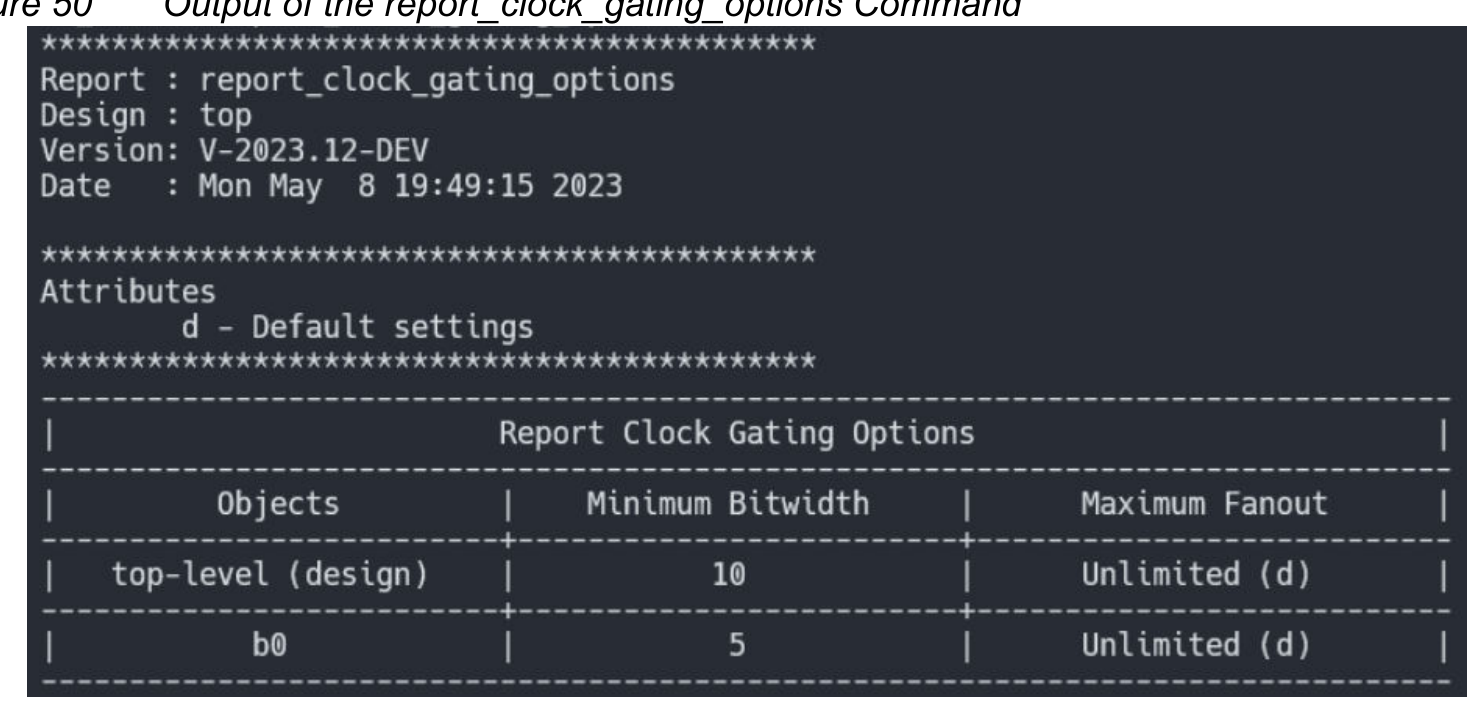
\includegraphics[width=0.92\textwidth,keepaspectratio]{figures/fig-cg-rpto-opts.png}
\caption{\cmd{report\_clock\_gating\_options} 命令输出}
\label{fig:cg-rpto-opts}
\end{figure}

当未设置任何门控选项，或设计仅设置了特定选项时，表在单行中显示已分配选项，以及可能通过 \opt{-objects} 参数传入的其他对象。

图~\ref{fig:cg-rpto-no-obj} 给出未对特定对象设置选项时 \cmd{report\_clock\_gating\_options} 的输出。

\begin{figure}[htbp]
\centering
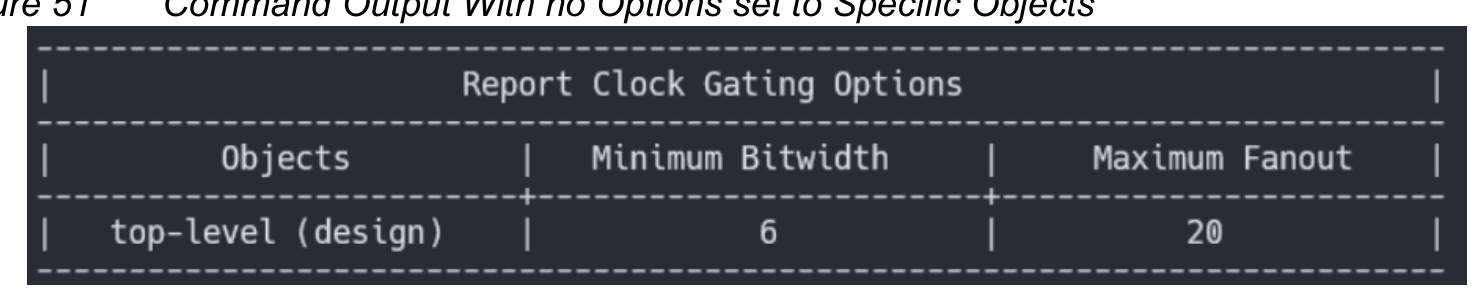
\includegraphics[width=0.92\textwidth,keepaspectratio]{figures/fig-cg-rpto-no-obj.png}
\caption{未对特定对象设置选项时的命令输出}
\label{fig:cg-rpto-no-obj}
\end{figure}

图~\ref{fig:cg-rpto-params} 给出未对特定对象设置选项、但将设计与 \texttt{b0} 均作为 objects 参数传入时的输出。

\begin{figure}[htbp]
\centering
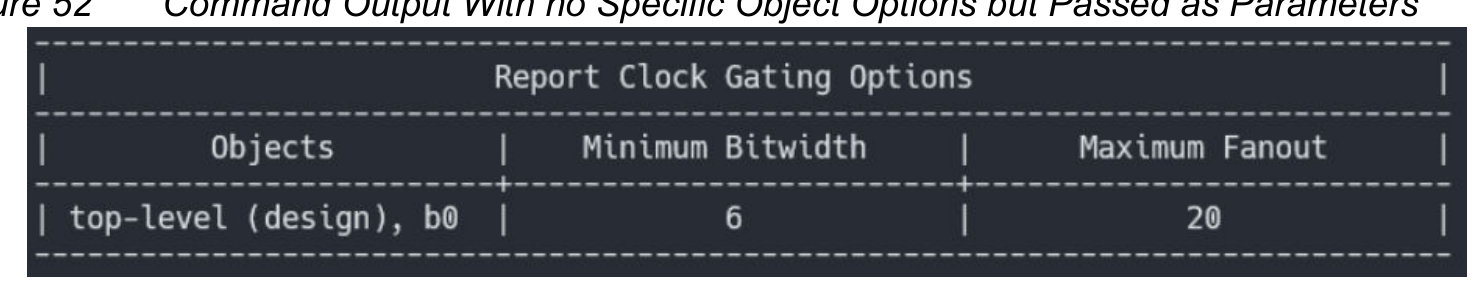
\includegraphics[width=0.92\textwidth,keepaspectratio]{figures/fig-cg-rpto-params.png}
\caption{无特定对象选项但作为参数传入时的命令输出}
\label{fig:cg-rpto-params}
\end{figure}

当多个对象用相同选项设置时，它们出现在同一行；若未使用 \opt{-nosplit} 参数，名称列会分成多行；否则全部占单行。
\begin{lstlisting}
report_clock_gating_options -objects {design, obj1, obj2, obj3, obj4}
\end{lstlisting}

\begin{figure}[htbp]
\centering
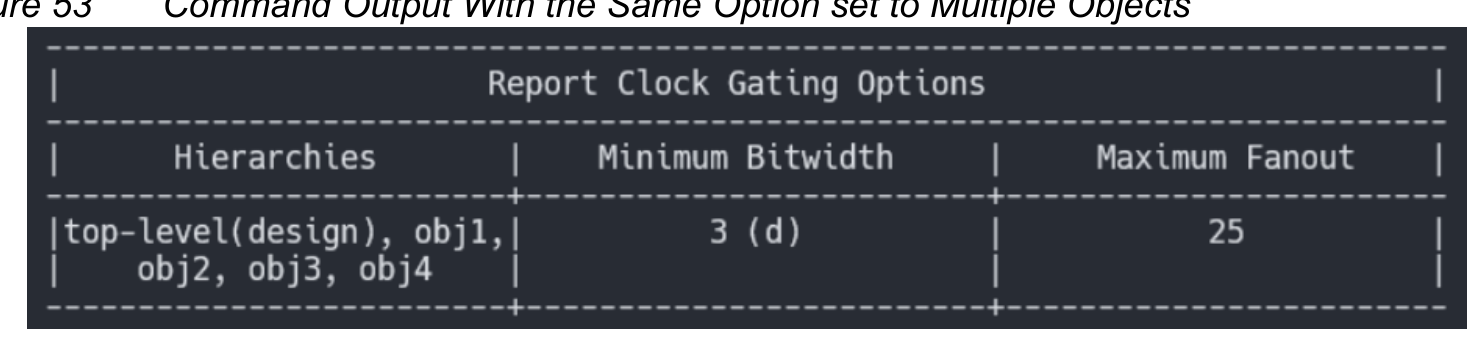
\includegraphics[width=0.92\textwidth,keepaspectratio]{figures/fig-cg-rpto-same.png}
\caption{多个对象设置相同选项时的命令输出}
\label{fig:cg-rpto-same}
\end{figure}

图~\ref{fig:cg-rpto-nosplit} 给出与图~\ref{fig:cg-rpto-same} 相同场景、但使用 \opt{-nosplit} 参数时的情况：
\begin{lstlisting}
report_clock_gating_options -objects {design, obj1, obj2, obj3, obj4} \
 -nosplit
\end{lstlisting}

\begin{figure}[htbp]
\centering
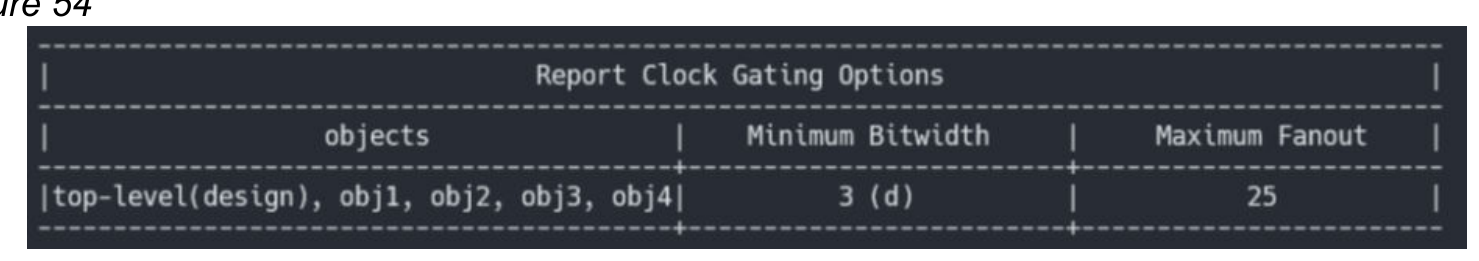
\includegraphics[width=0.92\textwidth,keepaspectratio]{figures/fig-cg-rpto-nosplit.png}
\caption{使用 \opt{-nosplit} 时的命令输出}
\label{fig:cg-rpto-nosplit}
\end{figure}

% ============================================================
\section{时钟门控流程}
\subsection*{Clock Gating Flows}

Fusion Compiler 工具在 \cmd{compile\_fusion} 命令期间插入时钟门控单元。下列主题描述时钟门控流程：
\begin{itemize}
  \item 在多电压设计中插入时钟门控（Inserting Clock Gates in Multivoltage Designs）
  \item 在 RTL 设计中插入时钟门控（Inserting Clock Gates in an RTL Design）
\end{itemize}

% ------------------------------------------------------------
\subsection{在多电压设计中插入时钟门控}
\subsubsection*{Inserting Clock Gates in Multivoltage Designs}

在多电压设计中，设计的不同层次可能具有不同工作条件，并使用不同的目标库子集。
在多电压设计中插入时钟门控单元时，工具根据指定的时钟门控风格，以及与设计层次单元工作条件匹配的工作条件，选择合适的库单元。
若未指定时钟门控风格，工具使用默认风格：测试点为 \texttt{before}，观察输出为 \texttt{false}。

若工具找不到同时适合时钟门控风格与工作条件的库单元，会发出警告消息且不插入时钟门控单元。
要检查是否有可用于时钟门控插入的集成时钟门控单元，使用 \cmd{check\_clock\_gate\_library\_cell\_availability} 命令。

% ------------------------------------------------------------
\subsection{在 RTL 设计中插入时钟门控}
\subsubsection*{Inserting Clock Gates in an RTL Design}

要在 RTL 设计中插入时钟门控逻辑并用该逻辑综合设计，按下列步骤操作：
\begin{enumerate}
  \item 读入 RTL 设计。
  \item （可选）用 \cmd{insert\_dft} 命令向设计插入测试单元。
  \item 用 \cmd{compile\_fusion} 命令编译设计。\\
    编译过程中，工具对符合时钟门控资格的寄存器插入时钟门控。
    默认情况下，\cmd{compile\_fusion} 在时钟门控插入期间使用时钟门控默认设置，并遵守逻辑库中指定的建立、保持及其他约束。
    要覆盖库中指定的建立与保持值，在编译设计前使用 \cmd{set\_clock\_gating\_check} 命令。默认设置适用于大多数设计。\\
    \cmd{compile\_fusion} 命令会按需自动连接集成时钟门控单元的 scan enable 与 test port 或 pin。
  \item 用 \cmd{report\_clock\_gating} 命令报告设计中的寄存器与时钟门控单元。用 \cmd{report\_power} 命令获取时钟门控插入后设计所用动态功耗信息。
\end{enumerate}

下例给出使用默认设置的典型命令序列：
\begin{lstlisting}
fc_shell> read_verilog design.v
fc_shell> create_clock -period 10 -name CLK
fc_shell> compile_fusion
fc_shell> insert_dft
fc_shell> report_clock_gating
fc_shell> report_power
\end{lstlisting}

% ============================================================
\section{替换时钟门控}
\subsection*{Replacing Clock Gates}

若希望用库中的集成时钟门控单元替换 RTL 中全部与工艺无关的时钟门控，在执行 \cmd{compile\_fusion} 之前使用 \cmd{replace\_clock\_gates} 命令。
\cmd{replace\_clock\_gates} 命令识别时钟网络中充当时钟门控的组合元件并加以替换。

使用 \cmd{replace\_clock\_gates} 时，工具在选择库单元时遵守 \cmd{set\_clock\_gate\_style}、\cmd{set\_lib\_cell\_purpose} 与 \cmd{set\_target\_library\_subset} 命令指定的约束。

当工具识别组合元件时，这些元件必须只有两个输入 pin（时钟 pin 与使能信号 pin）以及一个输出 pin。若不满足这些准则，该单元不是替换候选。
下表列出 WVGTECH 实例及其替换单元。

\begin{table}[htbp]
\centering
\caption{组合单元与集成时钟门控替换对照}
\label{tab:cg-replace}
\begin{tabularx}{\textwidth}{@{}l X@{}}
\toprule
\textbf{RTL 中的组合单元} & \textbf{集成时钟门控替换} \\
\midrule
AND 门 & 上升沿触发的基于锁存器的时钟门控 \\
OR 门 & 下降沿触发的基于锁存器的时钟门控 \\
NAND 门 & 下降沿触发的基于锁存器的时钟门控。时钟输入 pin 反相。 \\
NOR 门 & 下降沿触发的基于锁存器的时钟门控。两个输入 pin 均反相。 \\
\bottomrule
\end{tabularx}
\end{table}

新时钟门控单元按下列名称推断：
\begin{quote}
\texttt{rep\_clock\_gate\_+<instance\_name\_of\_combinational\_cell>}
\end{quote}

工具将已替换的时钟门控报告为工具插入的时钟门控。

% ============================================================
\section{控制时钟门控延迟}
\subsection*{Controlling Clock-Gate Latencies}

综合期间，Fusion Compiler 工具假定时钟为理想时钟（ideal clock）。理想时钟经时钟网络无延迟。
作此假定是因为真实时钟网络延迟要到时钟树综合之后才可知。
实际上时钟并非理想，经时钟网络存在非零延迟。
对于含时钟门控的设计，寄存器处的时钟网络延迟与时钟门控单元处不同。
寄存器与时钟门控单元之间时钟网络延迟的差异，会使时钟门控单元使能输入的建立条件约束更紧。

工具可通过下列方式获得时钟门控延迟：
\begin{itemize}
  \item \textbf{集成延迟估计（Integrated latency estimation）}\\
    默认情况下，工具在整个流程中估计并更新时钟门控延迟。估计的时钟延迟比用户指定的时钟延迟更准确。
  \item \textbf{用户指定延迟（User-specified latency）}\\
    可对特定实例禁用集成延迟估计，并手动指定延迟值。
\end{itemize}

% ------------------------------------------------------------
\subsection{集成时钟门控延迟估计}
\subsubsection*{Integrated Clock-Gate Latency Estimation}

默认情况下，工具在整个 \cmd{compile\_fusion} 命令流程中估计并更新时钟门控延迟。
这确保在时钟树综合之前时钟仍为理想时，工具在数据通路优化与有用偏斜（useful-skew）优化期间使用准确的时钟门控延迟。

若计划对设计执行结构化多源时钟树综合（structural multisource clock tree synthesis），请将 \appopt{opt.clock\_latency\_estimation.estimate\_smscts\_subtrees} 应用选项设为 \texttt{true}，以确保工具估计适合结构化多源时钟子树的时钟门控延迟。

为提高估计时钟门控延迟的准确性，在运行 \cmd{compile\_fusion} 之前指定时钟树综合设置，包括时钟树缓冲器库单元列表、时钟树反相器库单元列表以及时钟非默认布线规则。

估计的时钟延迟比用户指定的时钟延迟更准确。此外，工具在布局与多比特组库（multibit banking）等步骤之后更新估计的时钟延迟，而用户指定延迟是静态值。

要阻止工具估计特定时钟门控的延迟，用 \cmd{set\_attribute} 命令在其时钟 pin 上设置 \texttt{dont\_estimate\_clock\_latency} 属性，如下例：
\begin{lstlisting}
fc_shell> set_attribute \
   [get_pins {ICG21/CK}] dont_estimate_clock_latency true
\end{lstlisting}

为获得最佳结果，请勿将下列功能与集成时钟门控延迟估计一起使用：
\begin{itemize}
  \item 试探时钟树综合（Trial clock tree synthesis）\\
    要禁用此功能，将 \appopt{compile.flow.trial\_clock\_tree} 应用选项设为 \texttt{false}。
  \item 时钟门控优化（Clock-gate optimization）\\
    要禁用此功能，将 \appopt{compile.flow.optimize\_icgs} 应用选项设为 \texttt{false}。
  \item 布局感知时钟门控（Placement-aware clock gating）\\
    无论 \appopt{compile.clockgate.physically\_aware} 应用选项如何设置，启用时钟门控延迟估计时工具都会自动禁用此功能。
  \item 用户指定延迟\\
    用户指定延迟由 \cmd{set\_clock\_latency}、\cmd{set\_clock\_gate\_latency}、\cmd{set\_clock\_gating\_check -setup} 或 \cmd{set\_path\_margin -setup} 命令设置。
\end{itemize}

工具不会修改你在时钟门控单元上指定的任何 \cmd{set\_clock\_latency} 约束。
工具估计的时钟门控延迟值存储为相对用户指定值的偏移（offset）。
可用 \cmd{write\_script -format icc2} 命令查看偏移值，并在生成输出中检查 \cmd{set\_clock\_latency -offset} 命令。
若未设置任何延迟值，所报告偏移等于估计延迟值。

估计的延迟偏移值不会被捕获到 \cmd{write\_sdc} 命令生成的 SDC 文件中。

若时钟门控及其门控寄存器的相对位置在时钟树综合期间不变，延迟估计最准确。
要保留集成时钟门控的布局，在时钟树综合前将 \appopt{cts.compile.enable\_cell\_relocation} 应用选项设为 \texttt{auto}，以启用时钟网络单元的自动重定位。

% ------------------------------------------------------------
\subsection{用户指定时钟门控延迟}
\subsubsection*{User-Specified Clock-Gate Latency}

不能禁用总体的集成时钟门控延迟估计。但可通过在时钟 pin 上设置 \texttt{dont\_estimate\_clock\_latency} 属性，对特定时钟门控禁用该功能。
本节说明如何在这些时钟门控上手动指定延迟值。

用 \cmd{set\_clock\_latency} 或 \cmd{set\_clock\_gate\_latency} 命令指定时钟网络延迟。
\cmd{set\_clock\_gate\_latency} 命令可用于门级与 RTL 设计。

用 \cmd{set\_clock\_gate\_latency} 指定的时钟延迟，在 \cmd{compile\_fusion} 命令插入时钟门控单元时标注到寄存器上。
但若在编译后修改时钟门控上的延迟值，必须用 \cmd{apply\_clock\_gate\_latency} 命令手动将延迟值应用到已有时钟门控单元。

\begin{noteBox}
用 \cmd{set\_clock\_gate\_latency} 修改时钟门控延迟后，若再用 \cmd{compile\_fusion} 编译设计，无需用 \cmd{apply\_clock\_gate\_latency} 应用延迟值；工具会在编译期间标注指定值。
\end{noteBox}

要移除先前用 \cmd{set\_clock\_gate\_latency} 或 \cmd{apply\_clock\_gate\_latency} 在时钟门控单元上设置的时钟延迟信息，使用 \cmd{reset\_clock\_gate\_latency} 命令。
该命令移除指定时钟上的时钟延迟值。若不指定时钟，则移除全部时钟门控单元上的时钟延迟值。

% ------------------------------------------------------------
\subsection{set\_clock\_latency 命令}
\subsubsection*{The set\_clock\_latency Command}

用 \cmd{set\_clock\_latency} 命令为特定时钟门控单元指定时钟网络延迟。

在图~\ref{fig:cg-latency-design} 中，\texttt{lat\_cgtoreg} 是从时钟门控单元时钟 pin 到门控寄存器时钟 pin 的估计延迟，\texttt{lat\_reg} 是到无时钟门控寄存器时钟 pin 的估计时钟网络延迟。

\begin{figure}[htbp]
\centering
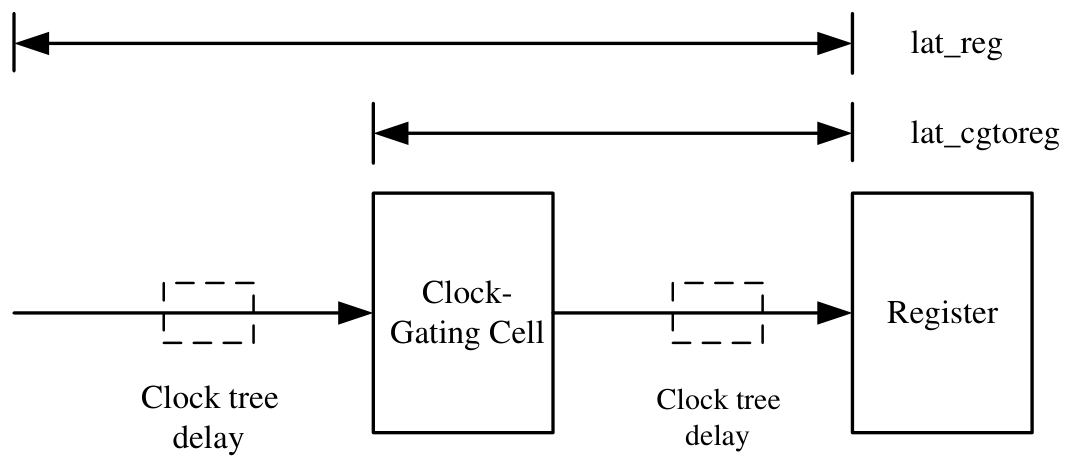
\includegraphics[width=0.92\textwidth,keepaspectratio]{figures/fig-clk-lat-cg.png}
\caption{含时钟门控设计的时钟延迟}
\label{fig:cg-latency-design}
\end{figure}

对于设计中由特定时钟驱动的全部寄存器（已门控或未门控）时钟 pin，对 \cmd{set\_clock\_latency} 使用 \texttt{lat\_reg} 值。
对全部时钟门控单元的时钟 pin，对 \cmd{set\_clock\_latency} 使用 \texttt{lat\_reg} 与 \texttt{lat\_cgtoreg} 之差。
由于设置延迟值的目的是计入寄存器与时钟门控单元之间不同的时钟网络延迟，重要的是获得差值（\texttt{lat\_cgtoreg}）的合理准确值。
除非用这些值处理与时钟门控无关的时钟网络延迟问题，否则绝对值本身并不那么重要。

% ------------------------------------------------------------
\subsection{set\_clock\_gate\_latency 命令}
\subsubsection*{The set\_clock\_gate\_latency Command}

使用 \cmd{compile\_fusion} 时，时钟门控在编译过程中插入。
要在工具插入时钟门控单元之前指定时钟网络延迟，使用 \cmd{set\_clock\_gate\_latency} 命令。
该命令允许将时钟门控单元的时钟网络延迟指定为时钟域、时钟门控阶段以及时钟门控单元扇出的函数。
你指定的延迟在 \cmd{compile\_fusion} 插入时钟门控单元时标注到其上。
也可用 \cmd{apply\_clock\_gate\_latency} 命令将延迟值手动标注到设计中已有的时钟门控单元。

\cmd{set\_clock\_gate\_latency} 命令接受下列参数：
\begin{itemize}
  \item \opt{-clock} \textit{clock\_list}
  \item \opt{-stage} \textit{clock\_gate\_stage}
  \item \opt{-fanout\_latency} \textit{fanout\_list}
\end{itemize}

\textit{fanout\_list} 是指定扇出范围与延迟减量的元组列表。
下例创建三个扇出范围：1 到 5，延迟值 0.5；6--15，延迟值 0.8；16 到无穷大，延迟值 0.6。
\begin{lstlisting}
set_clock_gate_latency -stage 1 \
      -fanout_latency {{1-5 0.5} {6-15 0.8} {16-inf 0.6}}
\end{lstlisting}

要为已时钟门控的寄存器指定时钟延迟值，将 \opt{-stage} 选项设为 0。
由于是为已时钟门控寄存器指定延迟值，\opt{-fanout\_latency} 的值应为 \texttt{1-inf}（1 到无穷大），且延迟是寄存器的绝对时钟延迟值，如下例：
\begin{lstlisting}
set_clock_gate_latency -clock CLK -stage 0 \
      -fanout_latency {1-inf 1.0}
\end{lstlisting}

若不指定 \opt{-clock}，设置应用于设计中全部时钟。

用 \cmd{set\_clock\_latency} 设置的时钟延迟优先级更高，不会被覆盖。

图~\ref{fig:cg-stage-latency} 给出时钟门控阶段与扇出的示例。

\begin{figure}[htbp]
\centering
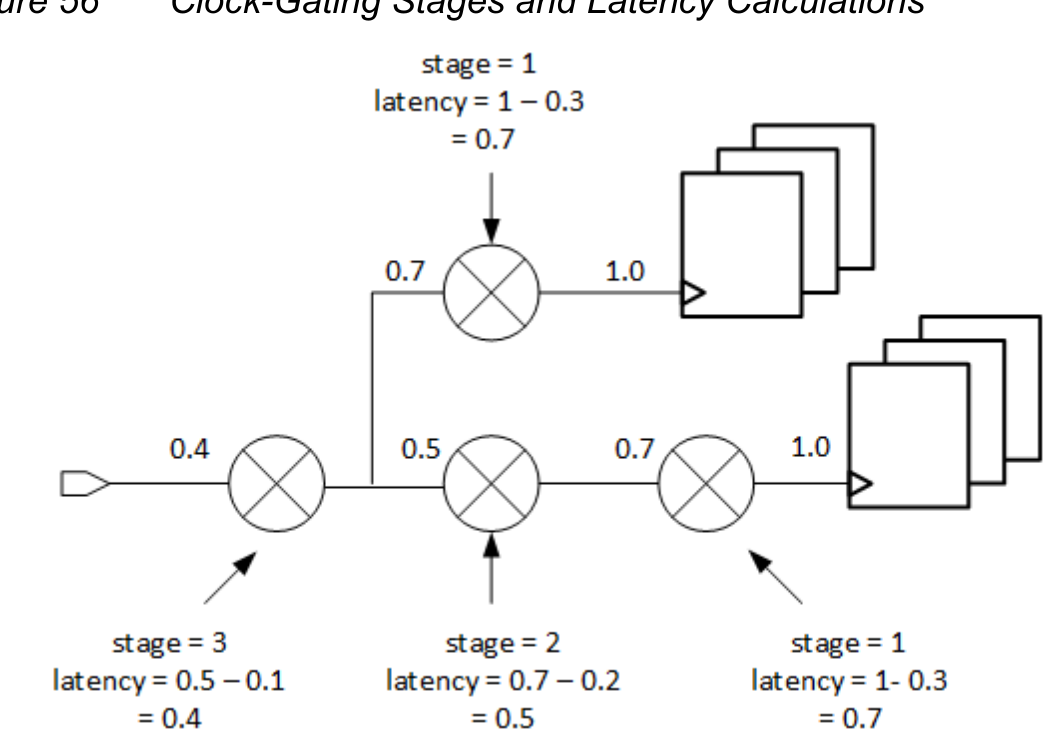
\includegraphics[width=0.70\textwidth,keepaspectratio]{figures/fig-cg-stages.png}
\caption{时钟门控阶段与延迟计算}
\label{fig:cg-stage-latency}
\end{figure}

下列命令为图~\ref{fig:cg-stage-latency} 设置延迟值：
\begin{lstlisting}
set_clock_gate_latency -stage 0 -fanout_latency {{1-inf 1.0}}
set_clock_gate_latency -stage 1 -fanout_latency {{1-inf 0.3}}
set_clock_gate_latency -stage 2 -fanout_latency {{1-inf 0.2}}
set_clock_gate_latency -stage 3 -fanout_latency {{1-inf 0.1}}
\end{lstlisting}

图~\ref{fig:cg-fanout-latency} 给出另一扇出与延迟计算示例。

\begin{figure}[htbp]
\centering
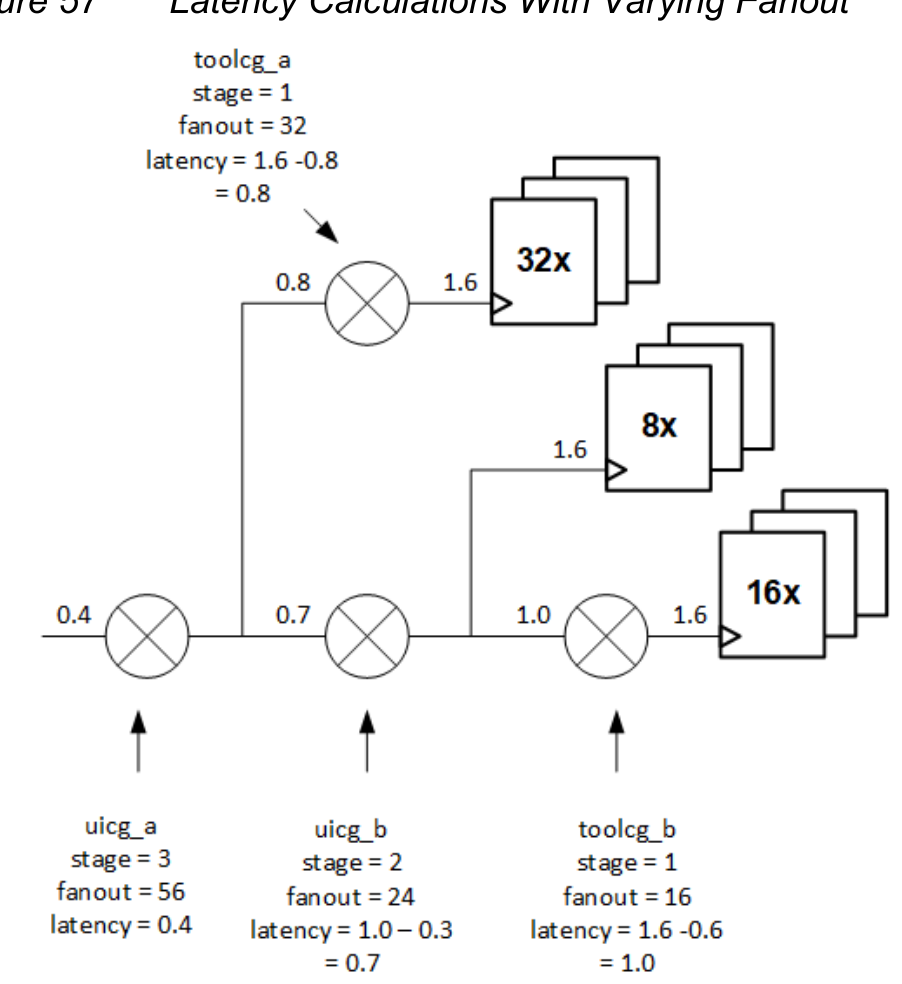
\includegraphics[width=0.55\textwidth,keepaspectratio]{figures/fig-lat-fanout.png}
\caption{变化扇出下的延迟计算}
\label{fig:cg-fanout-latency}
\end{figure}

下列命令为图~\ref{fig:cg-fanout-latency} 指定延迟与扇出：
\begin{lstlisting}
set_clock_gate_latency -stage 0 \
   -fanout_latency {{1-inf 1.6}}
set_clock_gate_latency -stage 1 \
   -fanout_latency {{1-20 0.6} {21-inf 0.8}}
set_clock_gate_latency -stage 2 \
   -fanout_latency {{1-20 0.2} {21-inf 0.3}}
set_clock_gate_latency -stage 3 \
   -fanout_latency {{1-30 0.1} {31-65 0.8} {66-inf 0.18}}
set_clock_latency "0.4" {uicg_a/CK}
\end{lstlisting}

注意：对时钟门控 \texttt{uicg\_a}，延迟值 0.4 由 \cmd{set\_clock\_latency} 赋值，不可被覆盖。

% ============================================================
\section{控制时钟门控级数}
\subsection*{Controlling the Number of Clock-Gate Levels}

时钟门控级数是时钟源与寄存器之间时钟门控的计数。
标准时钟门控插入提供一级时钟门控插入。
但设计中常含已有时钟门控，此时设计可能包含多级时钟门控。

可通过允许额外级数的时钟门控、限制时钟门控级数，或两者兼用，修改默认的时钟门控插入操作。

% ------------------------------------------------------------
\subsection{时钟门控多级扩展}
\subsubsection*{Clock-Gate Multilevel Expansion}

手动确定最佳时钟门控级数很难。Fusion Compiler 工具可分析全部时钟门控，并插入额外时钟门控以利用共享使能信号。
插入额外时钟门控可能改善功耗、面积或其他度量，取决于设计。
若六个或更多时钟门控共享使能信号，工具插入额外一级时钟门控。新时钟门控再被考虑进一步级数扩展。因此，该操作期间工具可能插入多级时钟门控。

要允许工具扩展时钟门控级数，将 \appopt{compile.clockgate.enable\_level\_expansion} 应用选项设为 \texttt{true}（默认为 \texttt{false}），并将 \appopt{compile.clockgate.max\_number\_of\_levels} 应用选项设为非零值（默认为 0）。
此时，工具添加时钟门控，直至满足下列任一条件：
\begin{itemize}
  \item 全部公共使能信号已识别并用于多级时钟门控扩展。
  \item 达到用户指定的最大时钟门控级数。
\end{itemize}

工具按下列方式命名新插入的时钟门控，取决于其使能函数被新时钟门控修改的那组时钟门控的状态：
\begin{itemize}
  \item 若至少一个时钟门控是工具插入的，基名为 \texttt{clock\_gate\_ml}。名称后附加寄存器基名，类似于其他工具插入时钟门控的命名约定。
  \item 若全部时钟门控都是已有的，工具使用扇出最大的已有时钟门控名称，并附加 \texttt{\_ml\_pe}。
\end{itemize}

\appopt{compile.clockgate.max\_number\_of\_levels} 应用选项指定允许的最大时钟门控级数。默认为 0，表示允许无穷多级。
但要使用时钟门控级数扩展能力，必须将该应用选项设为非零值（此外还需将 \appopt{compile.clockgate.enable\_level\_expansion} 设为 \texttt{true}）。

若指定了时钟门控级数扩展，但允许的最大级数偏低，扩展操作无法充分利用工具分析公共使能信号的能力。

要对特定时钟门控启用或禁用时钟门控级数扩展，使用 \cmd{set\_clock\_gate\_transformations -expand\_levels} 命令。

下列使用说明适用：
\begin{itemize}
  \item 新时钟门控继承由 \cmd{set\_clock\_gate\_transformations}、\cmd{set\_clock\_gate\_style}、\cmd{set\_dont\_touch}、\cmd{set\_size\_only}、\cmd{set\_lib\_cell\_purpose} 与 \cmd{set\_boundary\_optimization} 命令设置的约束。
  \item 插入操作后更新时钟门控延迟估计。
  \item 当插入操作修改某时钟门控的使能信号时，该门控保留其原有“已有”或“工具插入”的标识。
  \item 若已达到最大级数，自门控不得再添加另一级时钟门控。
  \item 多比特单元内的集成时钟门控计入时钟门控级数，但不是级数扩展候选。
  \item 新时钟门控不继承时序例外。
\end{itemize}

% ------------------------------------------------------------
\subsection{时钟门控折叠}
\subsubsection*{Clock-Gate Collapsing}

\appopt{compile.clockgate.max\_number\_of\_levels} 应用选项默认为 0，表示允许无穷多级。

可不启用时钟门控级数扩展而设置 \appopt{compile.clockgate.max\_number\_of\_levels}。
此时，若指定限值小于 \cmd{initial\_map} 阶段之后存在的时钟门控级数，工具会折叠（collapse）时钟门控级数。折叠方式如下：
\begin{itemize}
  \item 工具首先尝试折叠高于指定最大级数的时钟门控，从最高级（最靠近寄存器）的时钟门控开始。
  \item 若某特定时钟门控无法折叠，工具尝试折叠上游时钟门控，直至到达最低级（最靠近源）。折叠可跨层次进行。工具尽量保留父（上游）时钟门控。
  \item 工具移除其余不满足最大级数的全部时钟门控。
\end{itemize}

% ------------------------------------------------------------
\subsection{控制工具插入的时钟门控级数}
\subsubsection*{Controlling Tool-Inserted Clock-Gate Levels}

可指定工具应对全部时钟门控或仅工具插入时钟门控使用的最大级数。
若为全部时钟门控指定值，必须知道 RTL 设计中已有多少级时钟门控。
或者，可仅对工具插入时钟门控指定值。关于 Fusion Compiler 如何计数时钟门控级数的细节，见“时钟门控级数与阶段”。

要用下列互斥选项之一指定最大时钟门控级数，使用 \cmd{set\_clock\_gating\_tree\_options} 命令：
\begin{itemize}
  \item \opt{-max\_total\_levels} 指定全部时钟门控的最大级数。参数为大于或等于 1 的整数。
  \item \opt{-max\_tool\_inserted\_levels} 指定工具插入时钟门控的最大级数。参数为大于或等于 1 的整数。
\end{itemize}

要将时钟级数控制限制到特定时钟源，使用 \cmd{set\_clock\_gating\_tree\_options} 的 \opt{-clocks} 选项，其参数为时钟列表。

若在尝试满足最大时钟级数约束时某些时钟门控不可折叠，要允许移除时钟门控（亦称 ungating），使用 \opt{-ungate\_if\_not\_collapsible} 选项。

% ------------------------------------------------------------
\subsection{基于活动的优化}
\subsubsection*{Activity-Based Optimization}

若加载了 SAIF 文件，Fusion Compiler 工具会分析翻转活动，以评估是否扩展工具插入的时钟门控。该分析可防止插入不必要的时钟门控。

例如，在图~\ref{fig:cg-before-expand} 中，时钟门控 A1 与 A2 各为两条路径所共有，因此是多级扩展候选。

\begin{figure}[htbp]
\centering
\fbox{\parbox{0.85\textwidth}{\centering\vspace{1.2cm}
\textit{（原书 Figure 58：Before Clock-Gate Level Expansion）}
\vspace{1.2cm}}}
\caption{时钟门控级数扩展前}
\label{fig:cg-before-expand}
\end{figure}

但若时钟门控 A2 始终使能，其翻转率为 0、静态概率为 1。此时再增加一级时钟门控并无收益。最终配置如图~\ref{fig:cg-after-expand} 所示。

\begin{figure}[htbp]
\centering
\fbox{\parbox{0.85\textwidth}{\centering\vspace{1.2cm}
\textit{（原书 Figure 59：After Clock-Gate Level Expansion）}
\vspace{1.2cm}}}
\caption{时钟门控级数扩展后}
\label{fig:cg-after-expand}
\end{figure}

若启用时钟门控级数扩展，Fusion Compiler 默认执行活动驱动分析。
若无 SAIF 文件，将 \appopt{compile.clockgate.enable\_activity\_driven\_level\_expansion} 应用选项设为 \texttt{false}（默认为 \texttt{true}）以禁用此功能。

若禁用时钟门控级数扩展，工具忽略 \appopt{compile.clockgate.enable\_activity\_driven\_level\_expansion} 应用选项。

% ============================================================
\section{合并时钟门控}
\subsection*{Merging Clock Gates}

通过合并时钟门控，工具试图在最大化时钟门控覆盖的同时最小化时钟门控数量。
工具查找共享公共时钟与使能信号的时钟门控单元。该功能默认开启。

不同层次中时钟门控单元的扇出可移到公共祖先中的时钟门控单元，前提是没有限制阻止 port punching。
注意工具还会检查时钟门控风格与多电压约束。

带有 \texttt{dont\_touch} 或 \texttt{size\_only} 约束的时钟门控单元不被优化。

要禁用此功能，使用 \cmd{set\_clock\_gate\_transformations} 命令。

% ============================================================
\section{设置时钟门控变换}
\subsection*{Setting Clock Gating Transformations}

默认情况下，综合设计时自动进行时钟门控优化。
但你可定义设置，以允许或阻止对特定对象的时钟门控优化。

工具不对时钟门控加以区分。每个时钟门控，无论是已有还是工具插入，都受优化约束。

限制时钟门控优化的最简单方式是使用 \cmd{set\_dont\_touch} 与 \cmd{set\_size\_only} 命令。
这些命令通过阻止全部时钟门控的移除、合并与拆分，限制所有时钟门控优化。

更精细的方法是使用 \cmd{set\_clock\_gate\_transformations} 命令。
用此命令可对每个集成时钟门控设置特定约束，并控制可对该时钟门控执行哪些操作。

\cmd{set\_clock\_gate\_transformations} 命令提供下列选项：
\begin{itemize}
  \item \opt{-split\_fanout}\\
    设为 \texttt{false} 时，即使扇出大于允许的最大值，也阻止扇出拆分。该设置也阻止布局感知时钟门控执行的任何拆分。
  \item \opt{-merge\_equivalents}\\
    设为 \texttt{true} 时，允许将时钟门控与等价时钟门控合并。
  \item \opt{-collapse\_levels}\\
    设为 \texttt{false} 时，阻止折叠冗余时钟门控。
  \item \opt{-ungate\_fanout}\\
    设为 \texttt{true} 时，指定时钟门控扇出保持未门控。
  \item \opt{-reset}\\
    重置整个设计的全部时钟门控设置。
\end{itemize}

若在时钟门控实例或时钟门控库单元上设置了 \texttt{size\_only} 或 \texttt{dont\_touch} 属性，这些属性优先于 \cmd{set\_clock\_gate\_transformations} 指定的任何约束。

% ------------------------------------------------------------
\subsection{使用时钟门控变换的示例}
\subsubsection*{Example Using Clock Gating Transformations}

对图~\ref{fig:cg-xform-ex} 中的示例，假定设置下列限制：
\begin{lstlisting}
set_clock_gating_options -minimum_bitwidth 6
set_clock_gate_transformations [get_cells uicg_b*] true \
     -ungate_fanout false
set_clock_gate_transformations [get_cells uicg_c*] false
\end{lstlisting}

\begin{figure}[htbp]
\centering
\fbox{\parbox{0.85\textwidth}{\centering\vspace{1.5cm}
\textit{（原书 Figure 60：Example of Clock Gating Restrictions）}
\vspace{1.5cm}}}
\caption{时钟门控限制示例}
\label{fig:cg-xform-ex}
\end{figure}

优化期间，工具因最小位宽违例（最小位宽为 6）移除 \texttt{uicg\_a} 时钟门控。
\texttt{uicg\_b1} 与 \texttt{uicg\_b2} 时钟门控被合并（假定它们有等价使能信号）。
即使未满足最小位宽，也不允许 ungating，因此寄存器保持门控。
\texttt{uicg\_c1} 与 \texttt{uicg\_c2} 时钟门控不允许任何变换，因此不对这些时钟门控执行优化。

% ============================================================
\section{为时钟门控设置布线规则}
\subsection*{Setting Routing Rules for Clock Gates}

在设置物理实现约束时，可为特定 net 设置非默认布线规则，以定义更严格（更宽）的线宽与间距要求，从而改善时序并降低串扰。
要用 \cmd{create\_routing\_rule} 与 \cmd{set\_routing\_rule} 命令指定非默认布线规则。

但 \cmd{set\_routing\_rule} 命令不允许在工具插入时钟门控的输出 net 上标注，因为这些 net 要到执行 \cmd{compile\_fusion} 之后才存在。

要指定自动应用到工具插入时钟门控输出 pin 所连接 net 的非默认布线规则，使用 \cmd{set\_clock\_gate\_routing\_rule} 命令。这些规则在 \cmd{compile\_fusion} 命令之后应用到时钟门控。

例如：
\begin{lstlisting}
create_routing_rule cg_rule...
set_clock_gate_routing_rule -rule cg_rule
...
compile_fusion
...
report_routing_rules
\end{lstlisting}

% ============================================================
\section{时钟门控与多比特寄存器}
\subsection*{Clock Gating and Multibit Registers}

在 Fusion Compiler 流程中，时钟门控与多比特寄存器映射协同工作。多比特打包比率（multibit packing ratio）优先于时钟门控。

下列命令启用多比特映射：
\begin{lstlisting}
fc_shell> set_app_options -name compile.flow.enable_multibit -value true
\end{lstlisting}

不会插入时钟门控单元去门控预实例化的多比特寄存器。

关于时钟门控报告的更多信息，见“报告时钟门控结果”。

% ============================================================
\section{布局感知时钟门控}
\subsection*{Placement-Aware Clock Gating}

启用布局感知时钟门控时，工具执行下列优化：
\begin{itemize}
  \item 复制具有时序关键使能的时钟门控
  \item 调整时钟门控，使其更靠近所门控的寄存器
  \item 为时钟门控单元自动标注时钟网络延迟
\end{itemize}

要启用此功能，将 \appopt{compile.clockgate.physically\_aware} 应用选项设为 \texttt{true}。（默认为 \texttt{false}。）

图~\ref{fig:cg-phys-aware} 示例给出使用与不使用物理感知时钟门控的差异。在该布局视图中，可见集成时钟门控（红色显示）在物理上更靠近其门控寄存器。

\begin{figure}[htbp]
\centering
\fbox{\parbox{0.85\textwidth}{\centering\vspace{1.5cm}
\textit{（原书 Figure 61：Placement-Aware Clock Gating）}\\[0.3em]
\small 时钟门控单元红色；门控时钟 net 蓝色；Disabled vs Enabled 对比
\vspace{1.5cm}}}
\caption{布局感知时钟门控}
\label{fig:cg-phys-aware}
\end{figure}

% ============================================================
\section{基于扇入的时序时钟门控}
\subsection*{Fanin-Based Sequential Clock Gating}

时序时钟门控是从数据通路中上游或下游时序元件提取并传播使能条件，以便为额外寄存器启用时钟门控插入的过程。
Fusion Compiler 工具支持基于扇入的时序时钟门控：若传递扇入（transitive fanin）中的全部寄存器在上一时钟周期未改变状态，则某寄存器可在给定时钟周期被门控。

要启用此功能，将 \appopt{compile.clockgate.fanin\_sequential} 应用选项设为 \texttt{true}（默认为 \texttt{false}）。该功能需要 FC-New-Tech-Power 许可证。

图~\ref{fig:cg-seq-before} 与图~\ref{fig:cg-seq-after} 说明基于扇入的时序时钟门控的一般概念。
图~\ref{fig:cg-seq-before} 中的电路有寄存器组 R1，其传递扇入由寄存器组 R0 组成。
组 R0 中全部寄存器共享同一使能条件 EN0，且两组寄存器均由时钟 CLK 打拍。
若在某一时钟周期组 R0 中的寄存器被禁用（即使能信号 EN0 为 0），这些寄存器不改变取值。
因此，在下一时钟周期，组 R1 中的寄存器也不改变取值，从而成为时钟门控候选。

\begin{figure}[htbp]
\centering
\fbox{\parbox{0.85\textwidth}{\centering\vspace{1.2cm}
\textit{（原书 Figure 62：Before Clock Gating）}
\vspace{1.2cm}}}
\caption{时钟门控前}
\label{fig:cg-seq-before}
\end{figure}

图~\ref{fig:cg-seq-after} 给出时钟门控实现。首先为寄存器组 R0 插入时钟门控 CG1。
工具创建新寄存器 RD1 以生成使能信号 EN0 的延迟版本。延迟信号驱动寄存器组 R1 的时序时钟门控 SEQCG1。

\begin{figure}[htbp]
\centering
\fbox{\parbox{0.85\textwidth}{\centering\vspace{1.2cm}
\textit{（原书 Figure 63：After Clock Gating）}
\vspace{1.2cm}}}
\caption{时钟门控后}
\label{fig:cg-seq-after}
\end{figure}

Fusion Compiler 工具根据电路分析按需实现若干不同的时钟门控策略。
例如，若扇入寄存器并不都具有相同的使能信号，工具会在使能信号的上游查找公共信号，并将这些信号用作所插入延迟寄存器的输入。

时序时钟门控由 \cmd{compile\_fusion} 命令插入。
在 \cmd{initial\_map} 阶段，工具分析寄存器的局部层次并按需插入时钟门控。
在 \cmd{logic\_opto} 阶段，工具跨层次边界进行分析并按需插入额外时钟门控。

因基于扇入的时序时钟门控而插入的时钟门控，名称以 \texttt{seq\_clock\_gate\_fi\_} 为前缀，其余部分遵循标准时钟门控命名约定。
若因此功能插入延迟寄存器，寄存器名以 \texttt{reg\_seqcg\_} 为前缀，后接标准时钟门控命名约定（即被门控寄存器中最常见的基名）。

% ------------------------------------------------------------
\subsection{设置时序时钟门控选项}
\subsubsection*{Setting Sequential Clock Gating Options}

工具插入的时序时钟门控遵守 \cmd{set\_clock\_gate\_style} 命令中的设置（该命令适用于全部时钟门控）。
但下列命令专用于基于扇入的时序时钟门控：
\begin{itemize}
  \item \cmd{set\_fanin\_sequential\_clock\_gating\_options} 命令\\
    该命令指定基于扇入的时序时钟门控允许门控的最小位宽与最大扇出。默认最小位宽为 3，默认最大扇出无限制。可指定设置所应用的设计、电源域与层次实例列表。
  \item \cmd{report\_fanin\_sequential\_clock\_gating\_options} 命令\\
    该命令列出设计对象的设置。
  \item \cmd{set\_fanin\_sequential\_clock\_gating\_objects} 命令\\
    该命令允许指定要包含进或排除出基于扇入的时序时钟门控插入的寄存器、层次单元、电源域或模块。
  \item \cmd{report\_fanin\_sequential\_clock\_gating\_objects} 命令\\
    该命令列出用 \cmd{set\_fanin\_sequential\_clock\_gating\_objects} 显式设置的设置。
\end{itemize}

无论用 \cmd{set\_fanin\_sequential\_clock\_gating\_options} 与 \cmd{set\_fanin\_sequential\_clock\_gating\_objects} 做了何种设置，下列条件会阻止基于扇入的时序时钟门控插入：
\begin{itemize}
  \item 寄存器有异步状态变化。
  \item 寄存器的传递扇入包含边沿触发触发器以外的对象。禁止的对象包括 port、锁存器以及有异步状态变化的寄存器。
  \item 从传递扇入寄存器提取的使能信号依赖于其输出 pin。
  \item 寄存器时钟信号的翻转率过低，时钟门控无收益。
  \item 传递扇入中的寄存器由不同基时钟控制，或由相反时钟边沿触发。
  \item 传递扇入中至少一个寄存器始终使能。
  \item 所分析寄存器或其传递扇入寄存器的次态函数依赖于 RTL 中含 \texttt{dont\_care} 条件的逻辑。
  \item 所分析寄存器为多比特，且其切片不共享同一使能信号。
\end{itemize}

% ------------------------------------------------------------
\subsection{报告时序时钟门控}
\subsubsection*{Reporting Sequential Clock Gates}

若启用时序时钟门控，\cmd{report\_clock\_gating} 命令自动显示类似下表的汇总：
\begin{lstlisting}[caption={时序时钟门控汇总示例}]
Sequential Clock Gating Summary
------------------------------------------------------------------------------
|                                                             |   Bitwidth   |
------------------------------------------------------------------------------
|No of sequential clock gates                  |     2         |              |
|                                              |               |              |
|No of fanin-based sequential clock gates      |    2 (100.0%) |              |
|                                              |               |              |
|No of sequentially-gated registers            |    7 (21.2%)  |    7 (21.2%) |
|                                              |               |              |
|No of fanin-based sequentially-gated regs     |    7 (21.2%)  |    7 (21.2%) |
|                                              |               |              |
|No of registers not sequentially gated        |   26 (78.8%)  |   26 (78.8%) |
|                                              |               |              |
|Total number of registers                     |   33          |   33         |
------------------------------------------------------------------------------
\end{lstlisting}

用 \cmd{report\_clock\_gating -ungated} 命令报告未实现时序时钟门控的原因。报告类似如下：
\begin{lstlisting}
fc_shell> report_clock_gating -ungated

--------------------------------------------------------------------------
             Not fanin-based sequentially gated registers
--------------------------------------------------------------------------
   Register    |    Reason for not gating            | What's next?
--------------------------------------------------------------------------
 q2_reg[0]     | Register contains object different than edge-triggered
                 flip-flops in its transitive fanin  | Check the register
                                                       transitive fanin
 q2_reg[4]     | Register contains object different than edge-triggered
                 flip-flops in its transitive fanin  | Check the register
                                                       transitive fanin
 u/reg1_reg[2] | Register enable function is not a cover of the transitive
                 fanin enable function               | Check the register
                                                       enable condition
--------------------------------------------------------------------------
   Total                   7
\end{lstlisting}

% ============================================================
\section{报告时钟门控结果}
\subsection*{Reporting Clock-Gating Results}

编译设计后，可用 \cmd{report\_clock\_gating} 命令检查结果。示例如图~\ref{fig:cg-rpt}。

\begin{figure}[htbp]
\centering
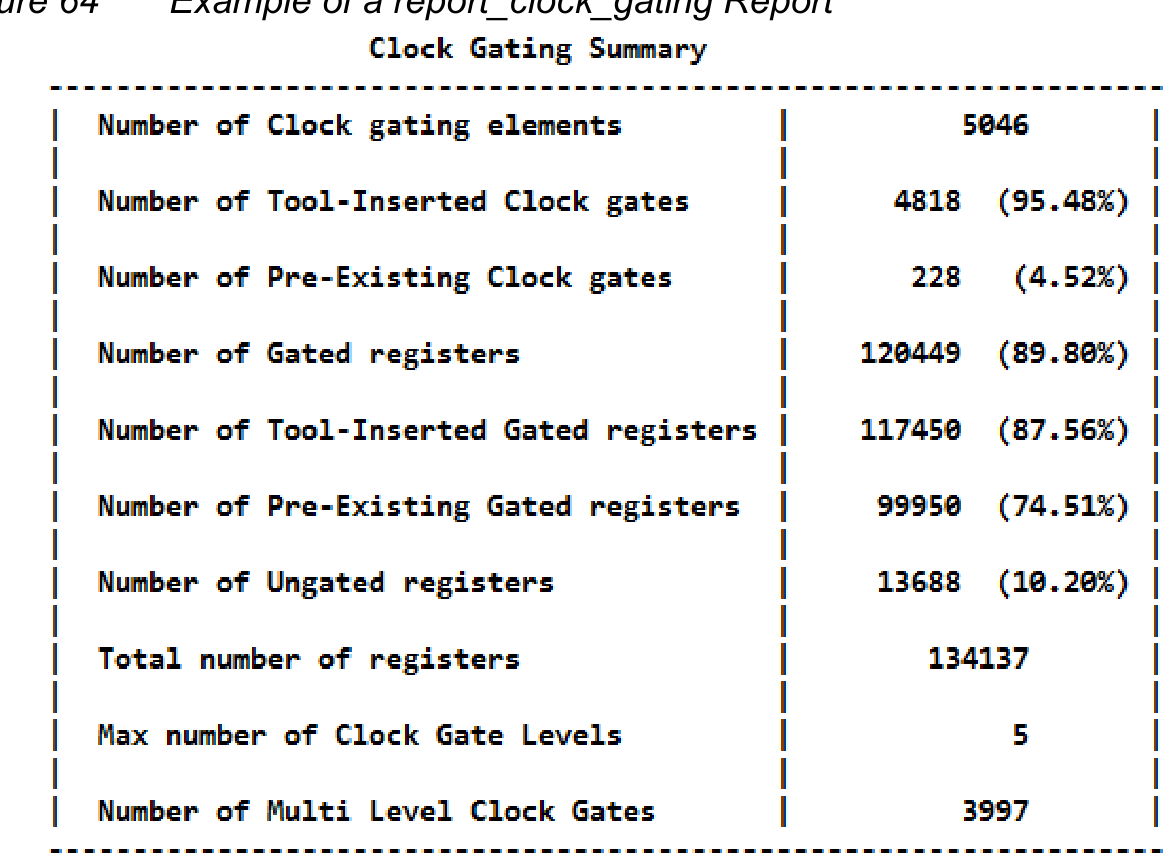
\includegraphics[width=0.72\textwidth,keepaspectratio]{figures/fig-cg-rpt.png}
\caption{\cmd{report\_clock\_gating} 报告示例}
\label{fig:cg-rpt}
\end{figure}

报告提供时钟门控统计汇总。“已有时钟门控（pre-existing clock gates）”指用户实例化的时钟门控。
已有类别也包括由工具插入时钟门控门控的寄存器。这包括同时由已有与工具插入时钟门控单元门控的寄存器。

默认情况下，工具报告多级统计，包括设计中时钟门控单元的最大级数。

时钟门控级数从时钟源向寄存器计数。

若设计中发现多比特触发器，会自动报告多比特组成（multibit composition）。

\begin{figure}[htbp]
\centering
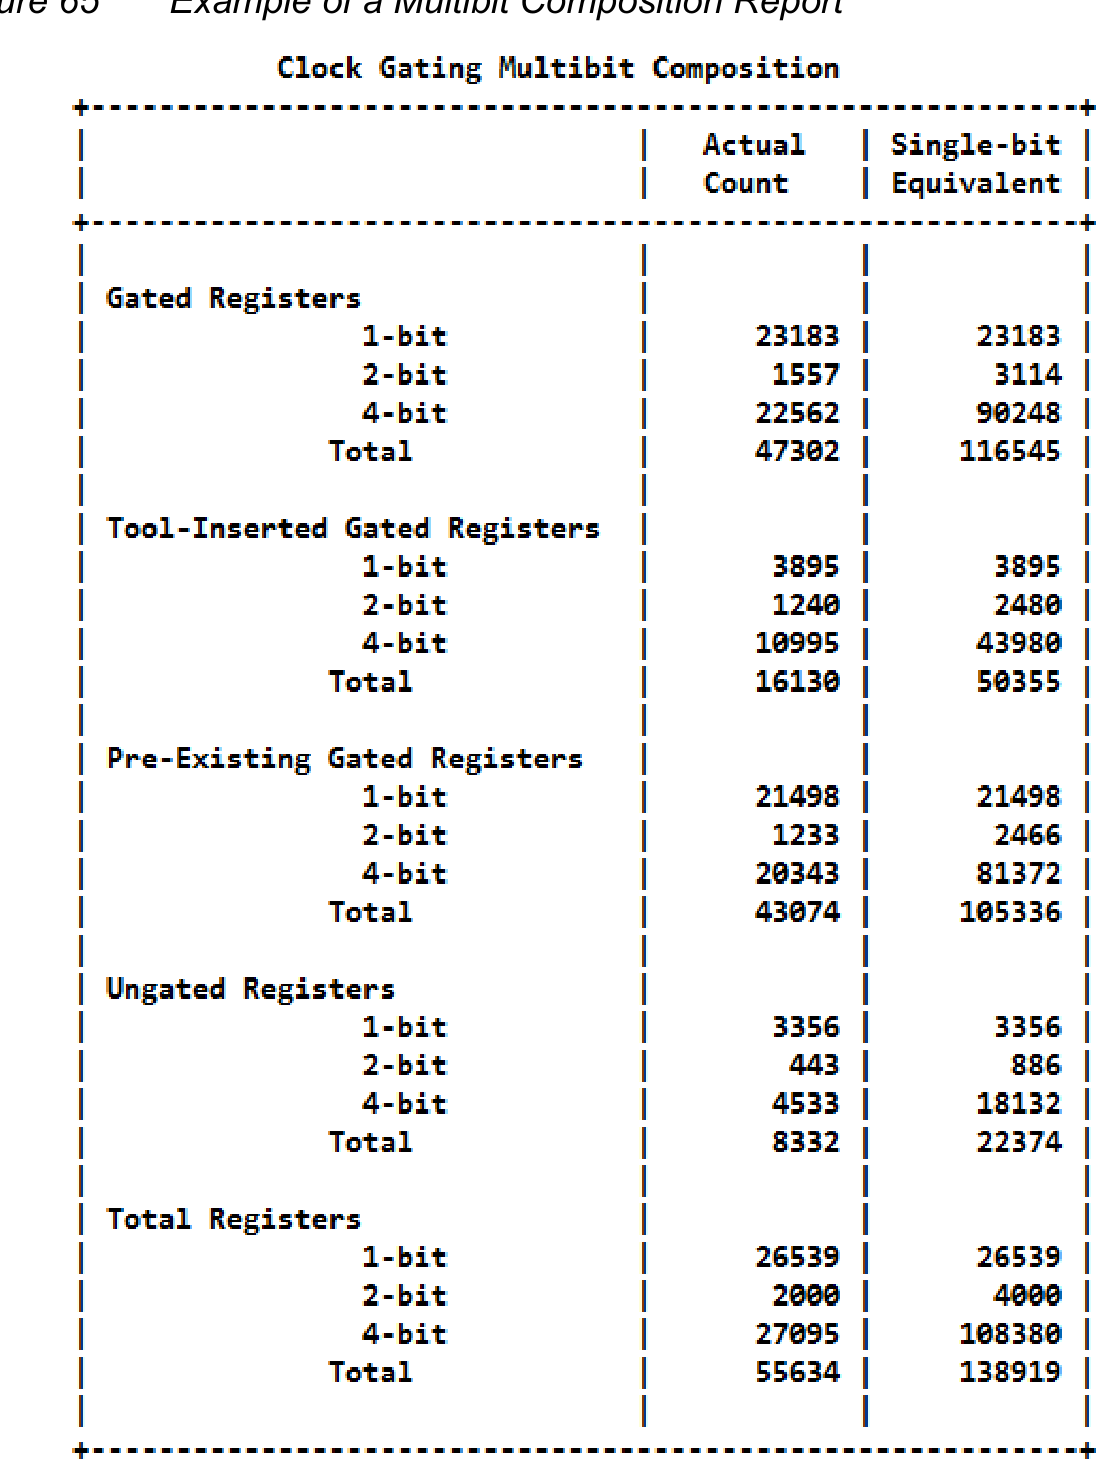
\includegraphics[width=0.55\textwidth,keepaspectratio]{figures/fig-cg-multibit-rpt.png}
\caption{多比特组成报告示例}
\label{fig:cg-multibit-rpt}
\end{figure}

要报告未门控寄存器的细节，对 \cmd{report\_clock\_gating} 使用 \opt{-ungated} 选项。要获取已门控寄存器的细节，使用 \opt{-gated} 选项。

% ============================================================
\section{报告时钟门控使能信号}
\subsection*{Reporting Clock-Gate Enable Signals}

时钟门控的使能信号通常是由下列一个或多个参考（或不变）点组成的布尔表达式：
\begin{itemize}
  \item 层次 port
  \item 时序输出 pin
  \item 黑盒输出 pin
\end{itemize}

要将时钟门控使能信号报告为布尔函数，使用 \cmd{report\_clock\_gating\_enable\_condition} 命令。必须指定要报告的时钟门控集合。

% ============================================================
\section{时钟门控效率报告}
\subsection*{Clock Gate Efficiency Reporting}

时钟门控效率报告功能通过考虑翻转率计算时钟门控效率。
该基于翻转率的计算与功耗节省直接相关，可用于改善门控效率。

\cmd{report\_clock\_gating\_efficiency} 命令报告用户指定时钟门控在每棵时钟树上的总体时钟门控效率。

命令语法如下：
\begin{lstlisting}
report_clock_gating_efficiency
[-by_register]
[-by_clock_gate]
[-bin_size]
[-type clock_gate | self_gate | fanin_seqcg]
[-origin tool_inserted | pre_existing]
[-sortby name | stage | gating_efficiency]
\end{lstlisting}

下图给出 \cmd{report\_clock\_gating\_efficiency} 命令报告：

\begin{figure}[htbp]
\centering
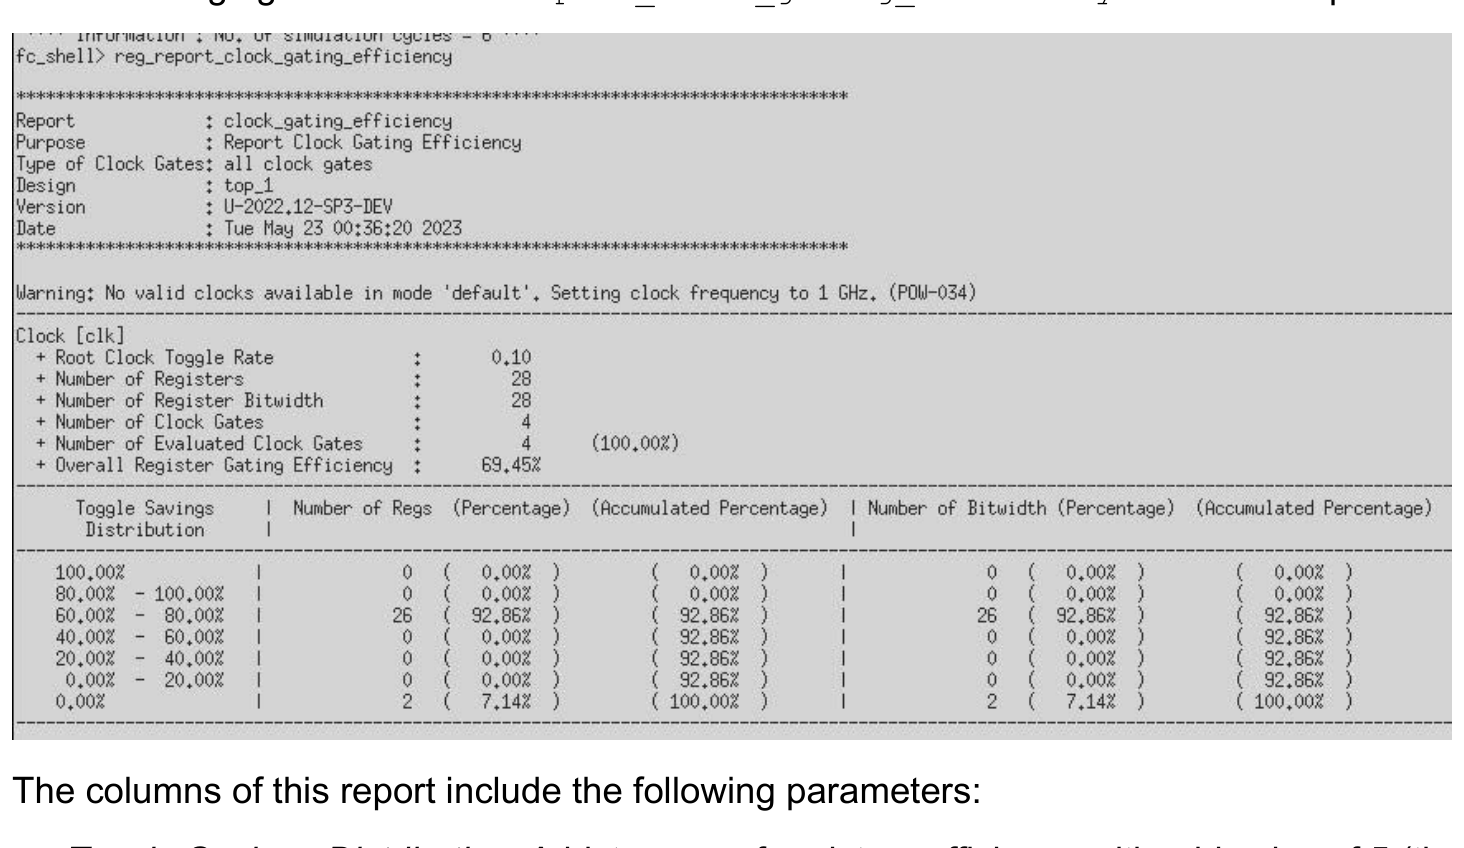
\includegraphics[width=0.92\textwidth,keepaspectratio]{figures/fig-cg-eff-rpt.png}
\caption{\cmd{report\_clock\_gating\_efficiency} 报告示例}
\label{fig:cg-eff-rpt}
\end{figure}

该报告的列包括下列参数：
\begin{itemize}
  \item \textbf{Toggle Savings Distribution}：寄存器效率直方图，bin 大小为 5（可修改）
  \item \textbf{Number of Registers}：每个直方图 bin 中的寄存器数
  \item \textbf{Accumulated Percentage}：迄今为止遇到的寄存器累计百分比
  \item \textbf{Number of Bitwidth}：每个 bin 中寄存器数的按位等价
  \item \textbf{Accumulated Percentage（of the bitwidth）}：迄今为止遇到的按位寄存器等价累计百分比
\end{itemize}

报告可按下列方式细化：
\begin{itemize}
  \item 用下列命令按 bin 大小报告效率：
\begin{lstlisting}
report_clock_gating_efficiency -bin_size #numberofbin
\end{lstlisting}
  \item 用下列命令按寄存器报告：
\begin{lstlisting}
report_clock_gating_efficiency -by_register
\end{lstlisting}
该报告的列包括：
  \begin{itemize}
    \item \textbf{Register}：所考虑寄存器的名称
    \item \textbf{Bitwidth}：寄存器位宽
    \item \textbf{Local Clock Toggle Rate}：门控后寄存器时钟 pin 上的翻转率
    \item \textbf{D Toggle Rate}：寄存器 D pin 上的翻转率
    \item \textbf{Q Toggle Rate}：寄存器 Q pin 上的翻转率
    \item \textbf{D/Clk Toggle Rate}：相对本地时钟翻转率的 D 翻转率
    \item \textbf{Q/Clk Toggle Rate}：相对本地时钟翻转率的 Q 翻转率
    \item \textbf{Current Gating Efficiency}：按 \(1 - (\text{local clock toggle} / \text{root clock toggle})\) 计算的寄存器效率
  \end{itemize}
  \item 用下列命令按时钟门控报告：
\begin{lstlisting}
report_clock_gating_efficiency -by_clock_gate
\end{lstlisting}
该报告的列包括：
  \begin{itemize}
    \item \textbf{Clock}：时钟门控的根时钟
    \item \textbf{Clock Gating Stage}：时钟门控阶段
    \item \textbf{Gating Element}
    \item \textbf{Number of Fanout Registers}：时钟门控直接驱动的寄存器数
    \item \textbf{Number of Fanout Bitwidth}：时钟门控直接驱动寄存器数的位宽等价
    \item \textbf{Toggle Savings}：时钟门控的翻转节省
    \item \textbf{Clock Gating Efficiency}：时钟门控效率
    \item \textbf{Receiver Clock Gate}：所考虑时钟门控直接驱动的时钟门控名称
  \end{itemize}
\end{itemize}

也可用下列命令按名称、效率或时钟门控阶段升序排序输出：
\begin{lstlisting}
report_clock_gating_efficiency -sort_by [name | stage | gating_efficiency]
\end{lstlisting}
\begin{itemize}
  \item \texttt{name}：按字母序
  \item \texttt{stage}：按时钟门控阶段
  \item \texttt{gating\_efficiency}：按时钟门控或寄存器门控效率
\end{itemize}

下图给出报告示例：

\begin{figure}[htbp]
\centering
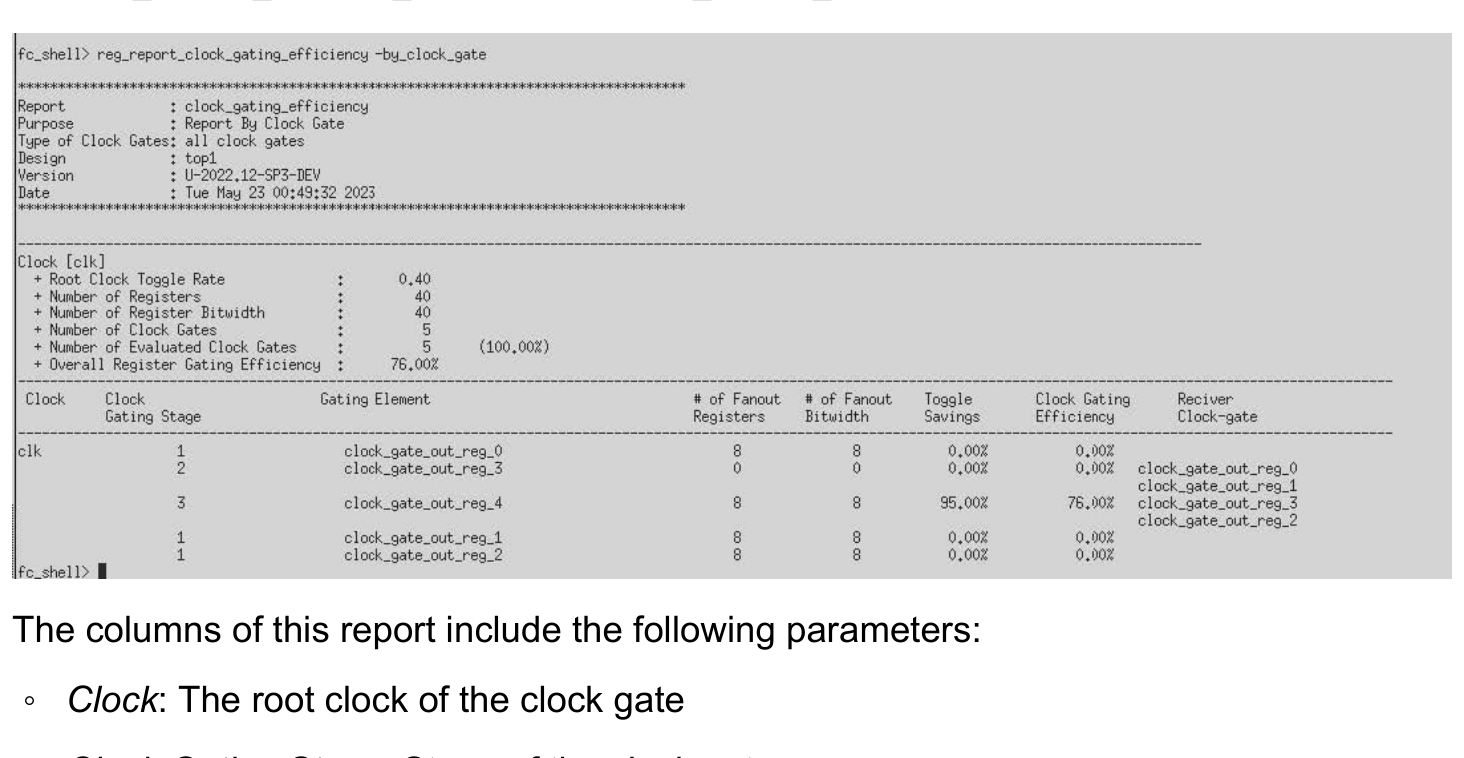
\includegraphics[width=0.92\textwidth,keepaspectratio]{figures/fig-cg-eff-by-cg.png}
\caption{时钟门控效率报告示例}
\label{fig:cg-eff-ex}
\end{figure}

% ============================================================
\section{自门控优化}
\subsection*{Self-Gating Optimization}

工具支持自门控优化，发生在 \cmd{compile\_fusion} 命令期间。
该功能在数据保持不变的时钟周期关闭某些寄存器的时钟信号，从而降低动态功耗。

\begin{figure}[htbp]
\centering
\fbox{\parbox{0.85\textwidth}{\centering\vspace{1.5cm}
\textit{（原书 Figure 66：Example of a Self-Gating Cell）}\\[0.3em]
\small CLK / D / Q 自门控单元示意
\vspace{1.5cm}}}
\caption{自门控单元示例}
\label{fig:cg-self-cell}
\end{figure}

无法从现有逻辑推断使能条件的寄存器，只能用自门控技术门控，不能用传统时钟门控。
默认情况下，工具仅对尚未门控的寄存器支持自门控。
可用 \cmd{set\_self\_gating\_options} 命令允许对这些寄存器进行自门控。
但对这些寄存器，时钟信号关闭的时间可能增加。

为确保 QoR 改善，自门控算法会考虑时序与功耗。若满足下列条件，则为寄存器插入自门控单元：
\begin{itemize}
  \item 寄存器数据 pin 有足够时序裕量。对多 scenario 设计，算法考虑为建立启用的活动 scenario 中最差情况的时序。
  \item 电路内部动态功耗降低。对多 scenario 设计，算法使用为动态功耗启用的活动 scenario 之间的平均内部动态功耗。
\end{itemize}

为最小化面积与功耗开销，可通过比较器单元树创建组合使能条件，使自门控单元在若干寄存器间共享。
若自门控寄存器由同步置位或同步清零信号驱动，这些信号也会纳入使能信号构造，使电路功能保持不变。
图~\ref{fig:cg-self-tree} 是跨两个寄存器（共 4 位）共享自门控单元的示例。
注意其中一个自门控寄存器是多比特寄存器，另一个是单比特寄存器。工具也可对多比特寄存器组或单比特寄存器组进行自门控。

\begin{figure}[htbp]
\centering
\fbox{\parbox{0.85\textwidth}{\centering\vspace{1.5cm}
\textit{（原书 Figure 67：Self-Gating Tree）}\\[0.3em]
\small CLK、D0/Q0、D1/Q1、D2/Q2、D/Q、EN 比较器树示意
\vspace{1.5cm}}}
\caption{自门控树}
\label{fig:cg-self-tree}
\end{figure}

工具不支持对下列类型的时序单元插入自门控：
\begin{itemize}
  \item 电平敏感时序单元
  \item 电平敏感扫描设计寄存器
  \item 主从触发器
  \item 保持寄存器（retention registers）
  \item 属于移位寄存器的单比特与多比特寄存器
  \item 具有多条时钟路径的多比特寄存器
\end{itemize}

更多信息见下列主题：
\begin{itemize}
  \item 自门控流程（Self-Gating Flow）
  \item 自门控的库要求（Library Requirements for Self-Gating）
  \item 自门控设置（Setting Up for Self-Gating）
  \item 报告与查询自门控单元（Reporting and Querying Self-Gating Cells）
\end{itemize}

% ------------------------------------------------------------
\subsection{自门控流程}
\subsubsection*{Self-Gating Flow}

图~\ref{fig:cg-self-flow} 说明用 \cmd{compile\_fusion} 命令插入自门控的 Fusion Compiler 流程。

\begin{figure}[htbp]
\centering
\fbox{\parbox{0.85\textwidth}{\centering\vspace{1.5cm}
\textit{（原书 Figure 68：General Self-Gating Flow）}\\[0.3em]
\small read\_saif / set\_switching\_activity $\to$ set\_app\_options compile.clockgate.self\_gating=true $\to$ compile\_fusion；输入 SAIF、RTL/netlist、Libraries；输出 Reports
\vspace{1.5cm}}}
\caption{一般自门控流程}
\label{fig:cg-self-flow}
\end{figure}

% ------------------------------------------------------------
\subsection{自门控的库要求}
\subsubsection*{Library Requirements for Self-Gating}

要执行自门控，逻辑库应包含 AND 与 OR 门以构建自门控树。库还应包含 XOR、NAND 与 OR 门用于比较器门。
库中的集成时钟门控单元必须具有下列设置：
\begin{itemize}
  \item 时序单元：latch
  \item 控制点：before
  \item 控制信号：scan\_enable
  \item 观察点：none
\end{itemize}

若库在对应工作条件下不含具有这些配置的单元，工具不插入自门控单元。
若用 \cmd{set\_clock\_gate\_style} 指定了与自门控兼容的集成时钟门控，自门控功能使用同一集成时钟门控，或与所指定最相似的时钟门控。

% ------------------------------------------------------------
\subsection{自门控设置}
\subsubsection*{Setting Up for Self-Gating}

要为块设置自门控，在运行 \cmd{compile\_fusion} 之前执行下列步骤：
\begin{enumerate}
  \item 将 \appopt{compile.clockgate.self\_gating} 应用选项设为 \texttt{true} 以启用自门控。
\begin{lstlisting}
fc_shell> set_app_options -name compile.clockgate.self_gating \
            -value true
\end{lstlisting}
  \item 用 \cmd{read\_saif} 或 \cmd{set\_switching\_activity} 命令施加翻转活动。
  \item （可选）用 \cmd{set\_self\_gating\_options} 命令指定自门控设置。更多信息见“设置自门控选项”。
  \item （可选）用 \cmd{set\_self\_gating\_objects} 命令覆盖工具选择自门控对象的默认行为。更多信息见“控制自门控对象的选择”。
\end{enumerate}

% ------------------------------------------------------------
\subsection{设置自门控选项}
\subsubsection*{Setting Self-Gating Options}

要用下列选项指定自门控设置，使用 \cmd{set\_self\_gating\_options} 命令：
\begin{itemize}
  \item \opt{-min\_bitwidth} \textit{bitwidth}\\
    控制自门控组的最小尺寸。默认值为 4。
  \item \opt{-max\_bitwidth} \textit{bitwidth}\\
    控制自门控组的最大尺寸。默认值为 8。
  \item \opt{-interaction\_with\_clock\_gating} \textit{interaction\_type}\\
    由用户实例化时钟门控单元门控的寄存器是自门控候选。有效参数为 \texttt{none}（跳过由工具插入时钟门控门控的寄存器）、\texttt{insert}（默认；在已门控寄存器上插入自门控）与 \texttt{collapse}（若工具插入时钟门控在同一层次则折叠它们）。
  \item \opt{-objects} \textit{object\_list}\\
    指定选项应应用到所列对象。支持的对象为层次实例、电源域与设计。默认情况下设置应用于整个设计。
  \item \opt{-tree\_type} \textit{combinational\_logic\_type}\\
    用指定逻辑类型构建门控使能树。有效参数为 \texttt{xor}、\texttt{nand}、\texttt{or} 与 \texttt{auto}（默认）。
\end{itemize}

要报告自门控选项，使用 \cmd{report\_self\_gating\_options} 命令。

% ------------------------------------------------------------
\subsection{控制自门控对象的选择}
\subsubsection*{Controlling the Selection of Self-Gating Objects}

要覆盖选择自门控对象的默认行为，用下列选项使用 \cmd{set\_self\_gating\_objects} 命令：
\begin{itemize}
  \item \opt{-force} \textit{object\_list}\\
    指示工具对所列对象执行自门控，即使对象未通过内部检查。
  \item \opt{-exclude} \textit{object\_list}\\
    阻止工具对所列对象自门控，即使它们通过内部检查。
  \item \opt{-include} \textit{object\_list}\\
    指定所列对象应按 \cmd{set\_clock\_gating\_options} 设置的插入规则进行自门控。这是设计中全部寄存器的默认设置。
  \item \opt{-clear} \textit{object\_list}\\
    移除所列对象上的全部包含、排除与强制准则。
  \item \opt{-reset}\\
    移除先前由 \cmd{set\_self\_gating\_objects} 设置的全部配置。
  \item \opt{-tree\_type} \textit{combinational\_logic\_type}\\
    指定要使用的组合单元类型。有效参数为 \texttt{xor}（默认）、\texttt{or}、\texttt{nand} 与 \texttt{auto}。指定 \texttt{auto} 时，工具根据翻转活动信息自动决定使用何种比较逻辑。这可能有助于在优化功耗的同时减小面积。必须与 \opt{-include} 或 \opt{-force} 选项一起使用。
\end{itemize}

要报告自门控对象，使用 \cmd{report\_self\_gating\_objects} 命令。

% ------------------------------------------------------------
\subsection{报告与查询自门控单元}
\subsubsection*{Reporting and Querying Self-Gating Cells}

默认情况下，\cmd{report\_clock\_gating} 命令自动检测设计中自门控的存在，并在报告底部显示相应信息，如下例报告所示。

\begin{lstlisting}[caption={含自门控汇总的时钟门控报告}]
                     Clock Gating Summary
------------------------------------------------------------------
|  Number of Clock gating elements         |         5           |
|                                          |                     |
|  Number of Tool-Inserted Clock gates     |         5 (100.00%) |
|                                          |                     |
|  Number of Pre-Existing Clock gates      |         0   (0.00%) |
|                                          |                     |
|  Number of Gated registers               |        48 (100.00%) |
|                                          |                     |
|  Number of Tool-Inserted Gated registers |        48 (100.00%) |
|                                          |                     |
|  Number of Pre-Existing Gated registers  |         0   (0.00%) |
|                                          |                     |
|  Number of Ungated registers             |         0   (0.00%) |
|                                          |                     |
|  Total number of registers               |            48       |
|                                          |                     |
|  Max number of Clock Gate Levels         |             2       |
|                                          |                     |
|  Number of Multi Level Clock Gates       |             4       |
------------------------------------------------------------------
                        Self Gating Summary
---------------------------------------------------------
|    Number of self-gating cells        |       3        |
|                                       |                |
|    Number of self gated registers     |  20  (41.67%)  |
|                                       |                |
|    Number of registers not self-gated |  28  (58.33%)  |
|                                       |                |
|    Total number of registers          |      48        |
----------------------------------------------------------
\end{lstlisting}

自门控单元在时钟门控汇总表中也计为时钟门控。
在此例中，有两个时钟门控与三个自门控，共五个时钟门控元件。

可用 \cmd{get\_clock\_gates} 命令查找设计中的全部自门控。该命令返回时钟门控或自门控单元的集合。
例如，下列命令返回门控由 CLK 打拍的寄存器的自门控单元：
\begin{lstlisting}
fc_shell> get_clock_gates -clock CLK -type self-gate
\end{lstlisting}

% ============================================================
\section{DFT wrapper 时钟门控的特殊命名与查询}
\subsection*{Special Naming and Querying for DFT Wrapper Clock Gates}

DFT wrapper 时钟门控指仅驱动 DFT wrapper 单元的那些时钟门控。
无论其来源如何，时钟门控引擎都会在全部 DFT wrapper 时钟门控名称前加上 \texttt{dft\_wrapper\_} 前缀。
这有助于在自动测试图案生成（ATPG）期间识别驱动 wrapper 单元的特定时钟门控。

\begin{table}[htbp]
\centering
\caption{命令及其期望返回值}
\label{tab:cg-dft-query}
\small
\begin{tabularx}{\textwidth}{@{}>{\raggedright\arraybackslash}X >{\raggedright\arraybackslash}X@{}}
\toprule
\textbf{命令} & \textbf{期望返回值} \\
\midrule
\cmd{get\_clock\_gates -gating\_wrapper\_cells\_only}\\
（返回仅驱动 wrapper 单元的全部时钟门控）
  & \texttt{dft\_wrapper\_ICG} 与 \texttt{dft\_wrapper\_clock\_gate\_reg} \\
\cmd{get\_clock\_gates -gating\_wrapper\_cells\_only -origin tool\_inserted}\\
（仅返回仅驱动 wrapper 单元的工具插入时钟门控）
  & 仅 \texttt{dft\_wrapper\_clock\_gate\_reg} \\
\cmd{get\_clock\_gates -gating\_wrapper\_cells\_only -origin pre\_existing}\\
（仅返回仅驱动 wrapper 单元的已有时钟门控）
  & 仅 \texttt{dft\_wrapper\_ICG} \\
\cmd{get\_clock\_gates \{ICG clock\_gate\_reg\} -gating\_wrapper\_cells\_only}
  & 空字符串，表示这两个时钟门控都不门控 wrapper 单元 \\
\cmd{get\_clock\_gates \{ICG dft\_wrapper\_clock\_gate\_reg\} -gating\_wrapper\_cells\_only}\\
（从 \{\} 括号内给定单元中返回仅驱动 wrapper 单元的时钟门控）
  & \texttt{dft\_wrapper\_clock\_gate\_reg} \\
\cmd{get\_clock\_gates \{*clock\_gate\_reg\} -gating\_wrapper\_cells\_only}\\
（返回仅驱动 wrapper 单元且匹配 \{\} 括号内给定模式的时钟门控）
  & \texttt{dft\_wrapper\_clock\_gate\_reg} \\
\bottomrule
\end{tabularx}
\end{table}

此功能仅在启用 DFT wrapper 单元的时钟门控支持时有效。要为 DFT wrapper 单元启用时钟门控支持，将下列变量设为 \texttt{true}：
\begin{quote}
\appopt{compile.clockgate.enable\_dft\_wrapper\_cell\_support}
\end{quote}

下图说明如何拆分时钟门控，使不同时钟门控可分别门控内部单元与 wrapper 单元：

\begin{figure}[htbp]
\centering
\fbox{\parbox{0.85\textwidth}{\centering\vspace{1.2cm}
\textit{（原书 Figure 69：Splitting a Clock Gate to Internal Cells and Wrapper Cells）}
\vspace{1.2cm}}}
\caption{将时钟门控拆分为内部单元与 wrapper 单元}
\label{fig:cg-dft-split}
\end{figure}

\begin{figure}[htbp]
\centering
\fbox{\parbox{0.85\textwidth}{\centering\vspace{1.2cm}
\textit{（原书 Figure 70：Gating Internal Cells and Wrapper Cells Separately）}
\vspace{1.2cm}}}
\caption{分别门控内部单元与 wrapper 单元}
\label{fig:cg-dft-sep}
\end{figure}

\begin{noteBox}
仅为门控 wrapper 单元而克隆的时钟门控，从其父时钟门控继承名称并附加 \texttt{dft\_wrapper\_}。这不适用于仅驱动 wrapper 单元的自门控名称。
\end{noteBox}

表~\ref{tab:cg-dft-rename} 说明不同类型时钟门控如何重命名。

\begin{table}[htbp]
\centering
\caption{不同类型时钟门控如何重命名}
\label{tab:cg-dft-rename}
\begin{tabularx}{\textwidth}{@{}l l X@{}}
\toprule
\textbf{时钟门控类型} & \textbf{原名} & \textbf{新名} \\
\midrule
工具插入 & \texttt{clock\_gate\_reg} & \texttt{dft\_wrapper\_clock\_gate\_reg} \\
已有 & \texttt{icg\_0} & \texttt{dft\_wrapper\_icg\_0} \\
\bottomrule
\end{tabularx}
\end{table}

对 \cmd{get\_clock\_gates} 命令使用 \opt{-gating\_wrapper\_cells\_only} 选项，可返回仅驱动 wrapper 单元的全部时钟门控（自门控除外）。该选项可与已有选项结合使用。

用 \appopt{compile.clockgate.substring\_list\_for\_dft\_wrapper\_dont\_rename\_icgs} 应用选项可限制（仅驱动 wrapper 单元的）已有时钟门控的重命名。该选项接受字符串列表作为值。名称匹配应用选项中任一子串的时钟门控不会被重命名。

\begin{noteBox}
\appopt{compile.clockgate.substring\_list\_for\_dft\_wrapper\_dont\_rename\_icgs} 应用选项对 \opt{-gating\_wrapper\_cells\_only} 查询选项无影响。
\end{noteBox}

考虑下例：
\begin{lstlisting}
set_app_options -name \
 compile.clockgate.substring_list_for_dft_wrapper_dont_rename_icgs -value \
 {clk_gate_ctl clk_gate_snps}
\end{lstlisting}

这可防止对名称中含 \texttt{clk\_gate\_ctl} 或 \texttt{clk\_gate\_snps} 模式的任何已有时钟门控进行重命名，但仍可用 \cmd{get\_clock\_gates -gating\_wrapper\_cells\_only} 查询它们。
